\chapter{Sound Event Classification}

The task of sound event classification consists of categorize an audio recording into one of a set of predefined categories, by associating a textual descriptor. In this chapter two works belonging to this ``sub-category'' are shown. They are respectively: Snore Sounds Excitation Localization, which has been performed by using \textit{Scattering Transform} and Deep Neural Networks and Road Surface Roughness Classification from Acoustic Signals by means of Convolutional Neural Networks.

\section{Snore Sounds Excitation Localization}

\begin{figure}[h]
	\centering
	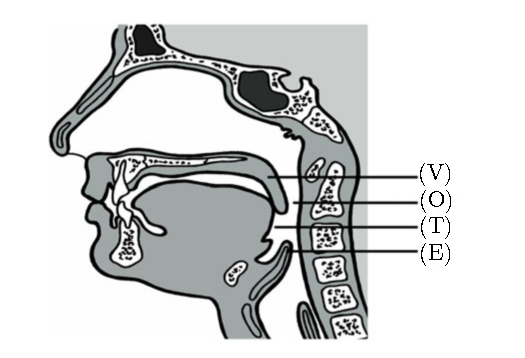
\includegraphics[width=0.6\linewidth]{img/vote.pdf}
	\caption[VOTE locations]{Corresponding positions of the VOTE classification in the upper airway. Picture courtesy of \cite{janott2014akustical}.} 
	\label{fig:vote}
\end{figure}

Snoring is defined as the emission, during the sleep, of a sound more or less annoying associated to the respiratory activity. This sound is caused by the vibration of soft tissue in the upper airways. It is confirmed that almost a half of the adult population snores occasionally, while approximately 30\% of the overall population suffers from chronic snoring almost every night \cite{young1997nasal}.
For this category of people, called habitual snorer, this disease can affect not only the sleep quality of the bed partner \cite{blumen2012snoring}, but it can also be associated with Obstructive Sleep Apnea (OSA), a chronic disease that can severely affect health \cite{strollo1996obstructive}. 
In fact, OSA  is an independent risk factor for cardiovascular diseases, stroke, hypertension, and myocardial infarction and in high-risk cases  a targeted medical intervention is necessary. Numerous surgical methods have been proposed to cure snoring, but many of them do not solve completely the issue if the origin of the vibration is not precisely located.
Although the exact mechanism of snoring sound generation is highly influenced by the individual anatomy, the typical areas from which the snore noise is produced have been located in the soft palate, the uvula, the palatine tonsils, the base of the tongue, and the epiglottis.
Drug induced sleep endoscopy (DISE) is a standard examination technique used to identify the location and form of vibrations and obstructions \cite{el2003predictive}. During a DISE procedure, a flexible nasopharyngoscope is introduced into the upper airways while the patient is in a state of artificial sleep. Vibration mechanisms and locations can be observed while video and audio signals are recorded. This procedure has several disadvantages: it is time consuming, the patient is put under strain, and it has to be performed during drug-induced sleep. 
Snoring carries information to the site and degree of obstruction of the upper airway \cite{pevernagie2010acoustics}, thus acoustic analysis of snoring sound could be an alternate, less-invasive method to identify the kind of snoring pathology \cite{schmitt2016bag}. It can be performed during natural sleep, avoiding the possibility to induce different muscle relaxation patterns which is a cause for possible diagnosis errors in drug-induced sleep.

\subsubsection{Related Works}
Several works have been presented in the recent years on multi-feature acoustic analysis methods with the aim to classify and segment snore/non-snore sleep sounds.
In \cite{cavusoglu2007efficient} the method is based on the characterization of spectral energy distribution of snoring signals and a two-dimensional projection via principal component analysis (PCA). In \cite{shokrollahi2016snoring} tracheal respiratory signals are recorded and snore segments are detected by extracting 10 temporal and spectral features and an Artificial Neural Network (ANN). In \cite{wang2016automatic} the automatic sound segmentation into snoring/breathing/noise episodes is performed using an adaptive effective-value threshold method for noise reduction, feature extraction of both linear and nonlinear descriptors and a Support Vector Machine (SVM) classifier.


Specifically regarding the determination of the vibration or occlusion mechanisms, the use of different acoustic feature sets has been proposed in \cite{janott2014akustical}, while in \cite{qian2015automatic} a k-nearest neighbor (k-NN) classifier is fed with different acoustic features. A performance comparison of different feature sets in combination with frequently-used classifier model is shown in \cite{qian2016classification}. 
Recently some works have been presented in occasion of the \textit{Snoring} task of the Interspeech 2017 Computational Paralinguistics Challenge (ComParE) \cite{ComParE2017}. The task consisted in identification of the snore type among four classes based on the widely used Velum-Oropharyngeal-Tongue-Epiglottis (VOTE) scheme, distinguishing four structures that can be involved in upper airway narrowing and obstruction. In  \cite{amiriparian2017snore, freitag2017end} the authors exploit deep convolutional neural networks pre-trained on image datasets for feature extraction from Short Time Fourier Transform (STFT) representation of the snore sounds. Then, the outputs of the bottom layers are used to feed a SVM model which provides the snore sound classification.
An alternative approach used weighted kernel classifiers \cite{kaya2017introducing} in order to counteract the natural snore dataset imbalance, such as Extreme Learning Machine and Kernel Partial Least Squares learners. Acoustic low level descriptors encoded over utterances are used as input features vector of the models. The latter algorithm is reported as the winner in the final challenge ratings\footnote{\url{http://emotion-research.net/sigs/speech-sig/is17-compare}}.


%\subsubsection{Contribution}
%
%In this work we propose a snore classification algorithm based on Deep Scattering Spectrum (SCAT) and Multi-layer Perceptron (MLP) neural networks. 
%
%The specific characteristic of the snore sounds and the references reported above demonstrate that typical techniques for speech analysis are required for an accurate classification, in particular feature vectors with high dimensionality. 
%In fact, the snore sound carries salient informations at different time scales, thus in this case it is necessary to capture patterns up to 500 ms. The Deep Scattering Spectrum (SCAT) \cite{anden2014deep} provides an efficient representation of an audio signal based on the scattering transform. In particular, it extends the traditional Mel-Frequency Cepstral Coefficients (MFCCs) representation  \cite{Davis80-COP}  with second-order scattering coefficients which characterize transient phenomena such as attacks and amplitude modulation.
%
%The acoustic spectral features extracted by means of the SCAT computation are pre-processed and mapped into Gaussian Mean Supervectors (GMS) \cite{Kinnunen2010} that are then used as input for the classifier. GMSs have been exploited with success in speech recognition \cite{principi2014power}, accent recognition \cite{bahari2013accent}, fall detection \cite{principi2016acoustic} and speaker recognition tasks \cite{Kinnunen2010}.  In particular, the SCAT of the input audio signal is computed and it is used to create a Universal Background Model (UBM) represented by a Gaussian Mixture Model (GMM) in the training phase. 
%GMS are extracted by adapting the GMM with the Maximum a Posteriori (MAP) algorithm and concatenating the mean value vectors. GMSs are finally employed for training the classifier. In the classification phase, the SCAT of the input audio signal is computed and it is used to calculate the GMS as in the training phase. The classifier, then, produces the final result. 
%
%The algorithms has been evaluated on the Munich-Passau Snore Sound Corpus (MPSSC) \cite{ComParE2017} and the results are expressed in terms of Unweighted Average Recall (UAR) in order to compare our approach with the results of the INTERSPEECH 2017 ComParE.



\subsection{Proposed approach}
In this work we propose a snore classification algorithm based on Deep Scattering Spectrum (SCAT) \cite{anden2014deep}  and Multi-layer Perceptron (MLP) neural networks. 
The specific characteristic of the snore sounds and the references reported above demonstrate that typical techniques for speech analysis are required for an accurate classification, in particular feature vectors with high dimensionality. 
In fact, the snore sound carries salient informations at different time scales, thus in this case it is necessary to capture patterns up to 500 ms. The SCAT provides an efficient representation of an audio signal based on the scattering transform. In particular, it extends the traditional Mel-Frequency Cepstral Coefficients (MFCCs) representation  \cite{Davis80-COP}  with second-order scattering coefficients which characterize transient phenomena such as attacks and amplitude modulation.
The algorithms has been evaluated on the Munich-Passau Snore Sound Corpus (MPSSC) \cite{ComParE2017} and the results are expressed in terms of Unweighted Average Recall (UAR) in order to compare our approach with the results of the INTERSPEECH 2017 ComParE.

The block diagram of the proposed method is shown in \figref{fig:scheme}. The algorithm operates by computing the deep scattering spectrum of the audio signal and then by mapping it into a GMS \cite{Kinnunen2010} for classification. In particular, referring to \figref{sfig:training}, the set of snoring sounds  $\mathcal{T}=\{(\mathbf{x}_1, C_1),(\mathbf{x}_2, C_2), \ldots,$ $ (\mathbf{x}_K, C_K)\}$  represents the training set of the algorithm, where $\mathbf{x}_k=[x_k(1), x_k(2),$ $\ldots, x_k(T_k)]$ is a snoring sound signal of length $T_k$ and $C_k \in \{V, O, T, E\}$ is the corresponding snoring label. 
The snore audio samples of the MPSSC corpus are of various duration ranging from 0.5 to 3 seconds, thus before computing the SCAT, audio signals shorter than 3\,s are padded to the same length equal to 3 seconds. Padding is performed by repeating a signal or part of it until the total amount of audio samples is equal to 48000. Then, by means of the Hamming window, the audio signals are divided into half overlapped frames ${x}_{k,l}[n] = {x}_{k}[n + l (N - P + 1) - P + 1]$, where $l$ is the frame index, $N=8000$ and $P=4000$.

In the ``SCAT'' stage every input audio signal $\mathbf{x}_{k}$ is converted into informative values that describe the main characteristics of the audio signal concatenating the scattering transform coefficients of each audio frame $SCAT({x}_{k,l})$, with $l=1,\dots,11$.
In the training phase, a Universal Background Model (UBM) represented by a Gaussian Mixture Model (GMM) is trained on the SCAT vectors computed on the set $\mathcal{T}$ by using the Expectation Maximisation algorithm. Then, the ``GMS Extraction'' block consists in adapting the UBM with the Maximum a Posteriori (MAP) algorithm  by using the SCAT of each snoring sound in $\mathcal{T}$ as input. The resulting mean values of each Gaussian of the GMM are concatenated into a GMS, thus mapping the SCAT coefficients time series into vectors of fixed lengths. %$\mathcal{G}=\{\mathbf{G}_1,\mathbf{G}_2, \ldots, \mathbf{G}_P\}$ is the set of GMS which is employed to train an SVM classifier. 
The final step of the training phase consists in training the Deep Neural Network (DNN) classifier. In this work we used a Multi-layer Perceptron neural network and we compared the performance with a state-of-the art approach such as Support Vector Machine (SVM).
In the classification phase (\figref{sfig:testing}), given a snore sound $\mathbf{x}_y$, the relative GMS is obtained from the UBM as in the training phase, and then it is fed to the classifier in order to find the corresponding label $C_y \in \{V, O, T, E\}$.



\begin{figure}[h]
	\centering
	\begin{subfigure}[b]{0.3\columnwidth}
		\def\svgwidth{\columnwidth}
		\input{4_sound_event_classification/scheme_train_v2.pdf_tex}
		\caption{Training.} \label{sfig:training}
	\end{subfigure}
	\begin{subfigure}[b]{0.3\columnwidth}
		\def\svgwidth{\columnwidth}
		\input{4_sound_event_classification/scheme_classify_v2.pdf_tex}
		\caption{Classification.} \label{sfig:testing}
	\end{subfigure}
	\caption{Scheme of the proposed approach.}\label{fig:scheme}
\end{figure}


\subsubsection{Deep Scattering Spectrum}

The scattering transform \cite{Mallat2012} is the operation on which the Deep Scattering Spectrum (SCAT) is based. SCAT is a multi-resolution representation of a signal based on a tree of complex wavelet filters followed by a non-linearity. The SCAT up to order $M$ of a signal $x_{k,l}$ is, thus, 
\begin{equation}
\begin{split}
\mathbf{S}(x_{k,l}, M) = & \{ x_{k,l} * \phi_M, \\
&  |x_{k,l} * \psi_{m_1} | * \phi_M, \\
&  ||x_{k,l} *  \psi_{m_1} | * \psi_{m_2}| * \phi_M \},
\end{split}
\end{equation}
where $\phi_M$ is a low-pass filter and $\psi_{m_i}$ is a wavelet filter with $i < M$. Time indices are omitted for brevity.
SCAT proves successful in gathering information at multiple resolutions on non-stationary signals thanks to its good properties, such as translation invariance up to level $M$, stability to small diffeomorphisms and uniqueness, e.g., time-warping deformations. It has been applied with success in image \cite{Sifre2013rotation} and audio signal classification tasks \cite{Anden2011multiscale}, where it is shown that SCAT provides optimal results when $M=2$ though there is no upper limit on the order of the SCAT. It is showed that a two orders cascade of wavelet filter banks and rectifiers improve results obtained by MFCC and Delta-MFCC descriptors in musical genre classification task, thus the energy remaining on higher order branching is as low as background noise and provides no additional information. The SCAT outputs time-averaged coefficients, providing informative signal invariants over potentially large time scales.
To compute the SCAT we used the \textit{ScatNet} open source \textsc{Matlab} library \cite{sifre2013scatnet}.
The choice of the wavelet filters is not trivial. In audio processing a typical procedure is to define constant-Q filter banks as linear operators that make up the layers of the scattering networks. The quality factors of the filter used in this work are $Q_1=8$ and $Q_2=1$.
We assume 0.5\,s as minimum length of snore utterance, thus the filter length $N$ is set equal to 8000 samples.

The wavelet functions are built by dilating a mother wavelet $\psi$ by a factor $2^{1/Q}$, for the quality factors $Q$, so as to obtain the filter bank:

\begin{equation}
\psi_{m_i}(t)= 2^{-m/Q} \psi(2^{-m/Q}t),
\end{equation}
with $t$ representing the time index.


\begin{figure}[h]
	\centering
	\begin{subfigure}[b]{0.45\columnwidth}
		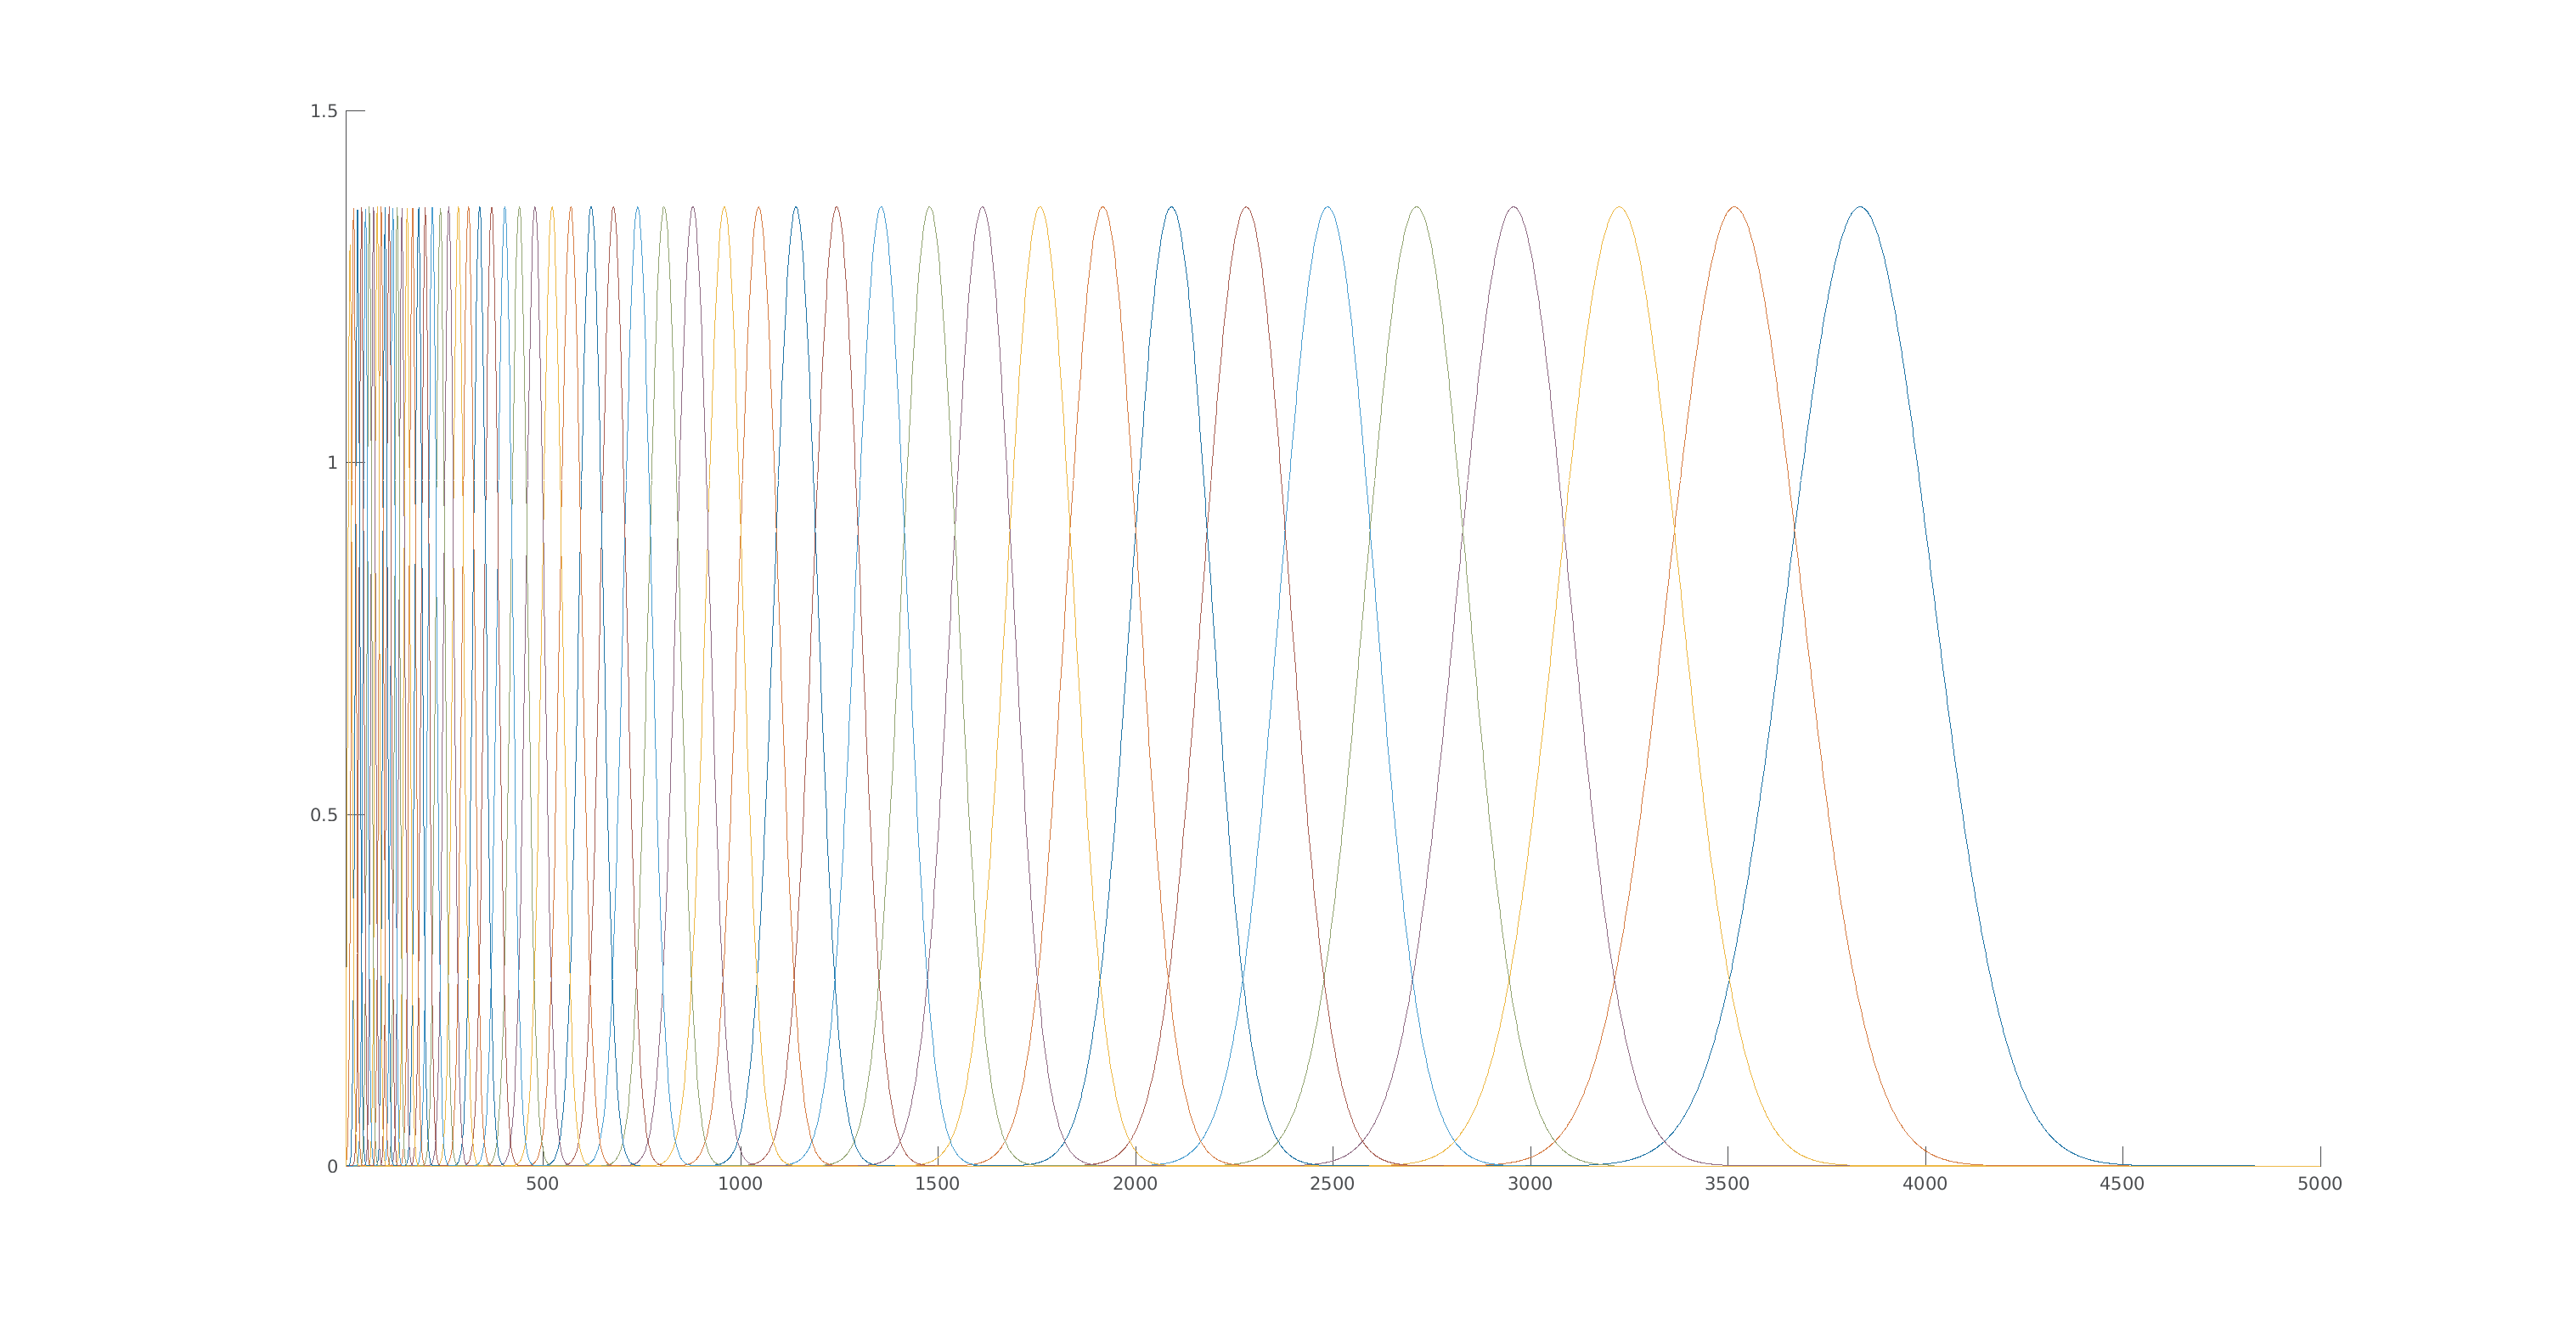
\includegraphics[width=0.9\textwidth]{img/scatter_filters_1.eps}
		\caption{First stage.}
	\end{subfigure}
	\begin{subfigure}[b]{0.45\columnwidth}
		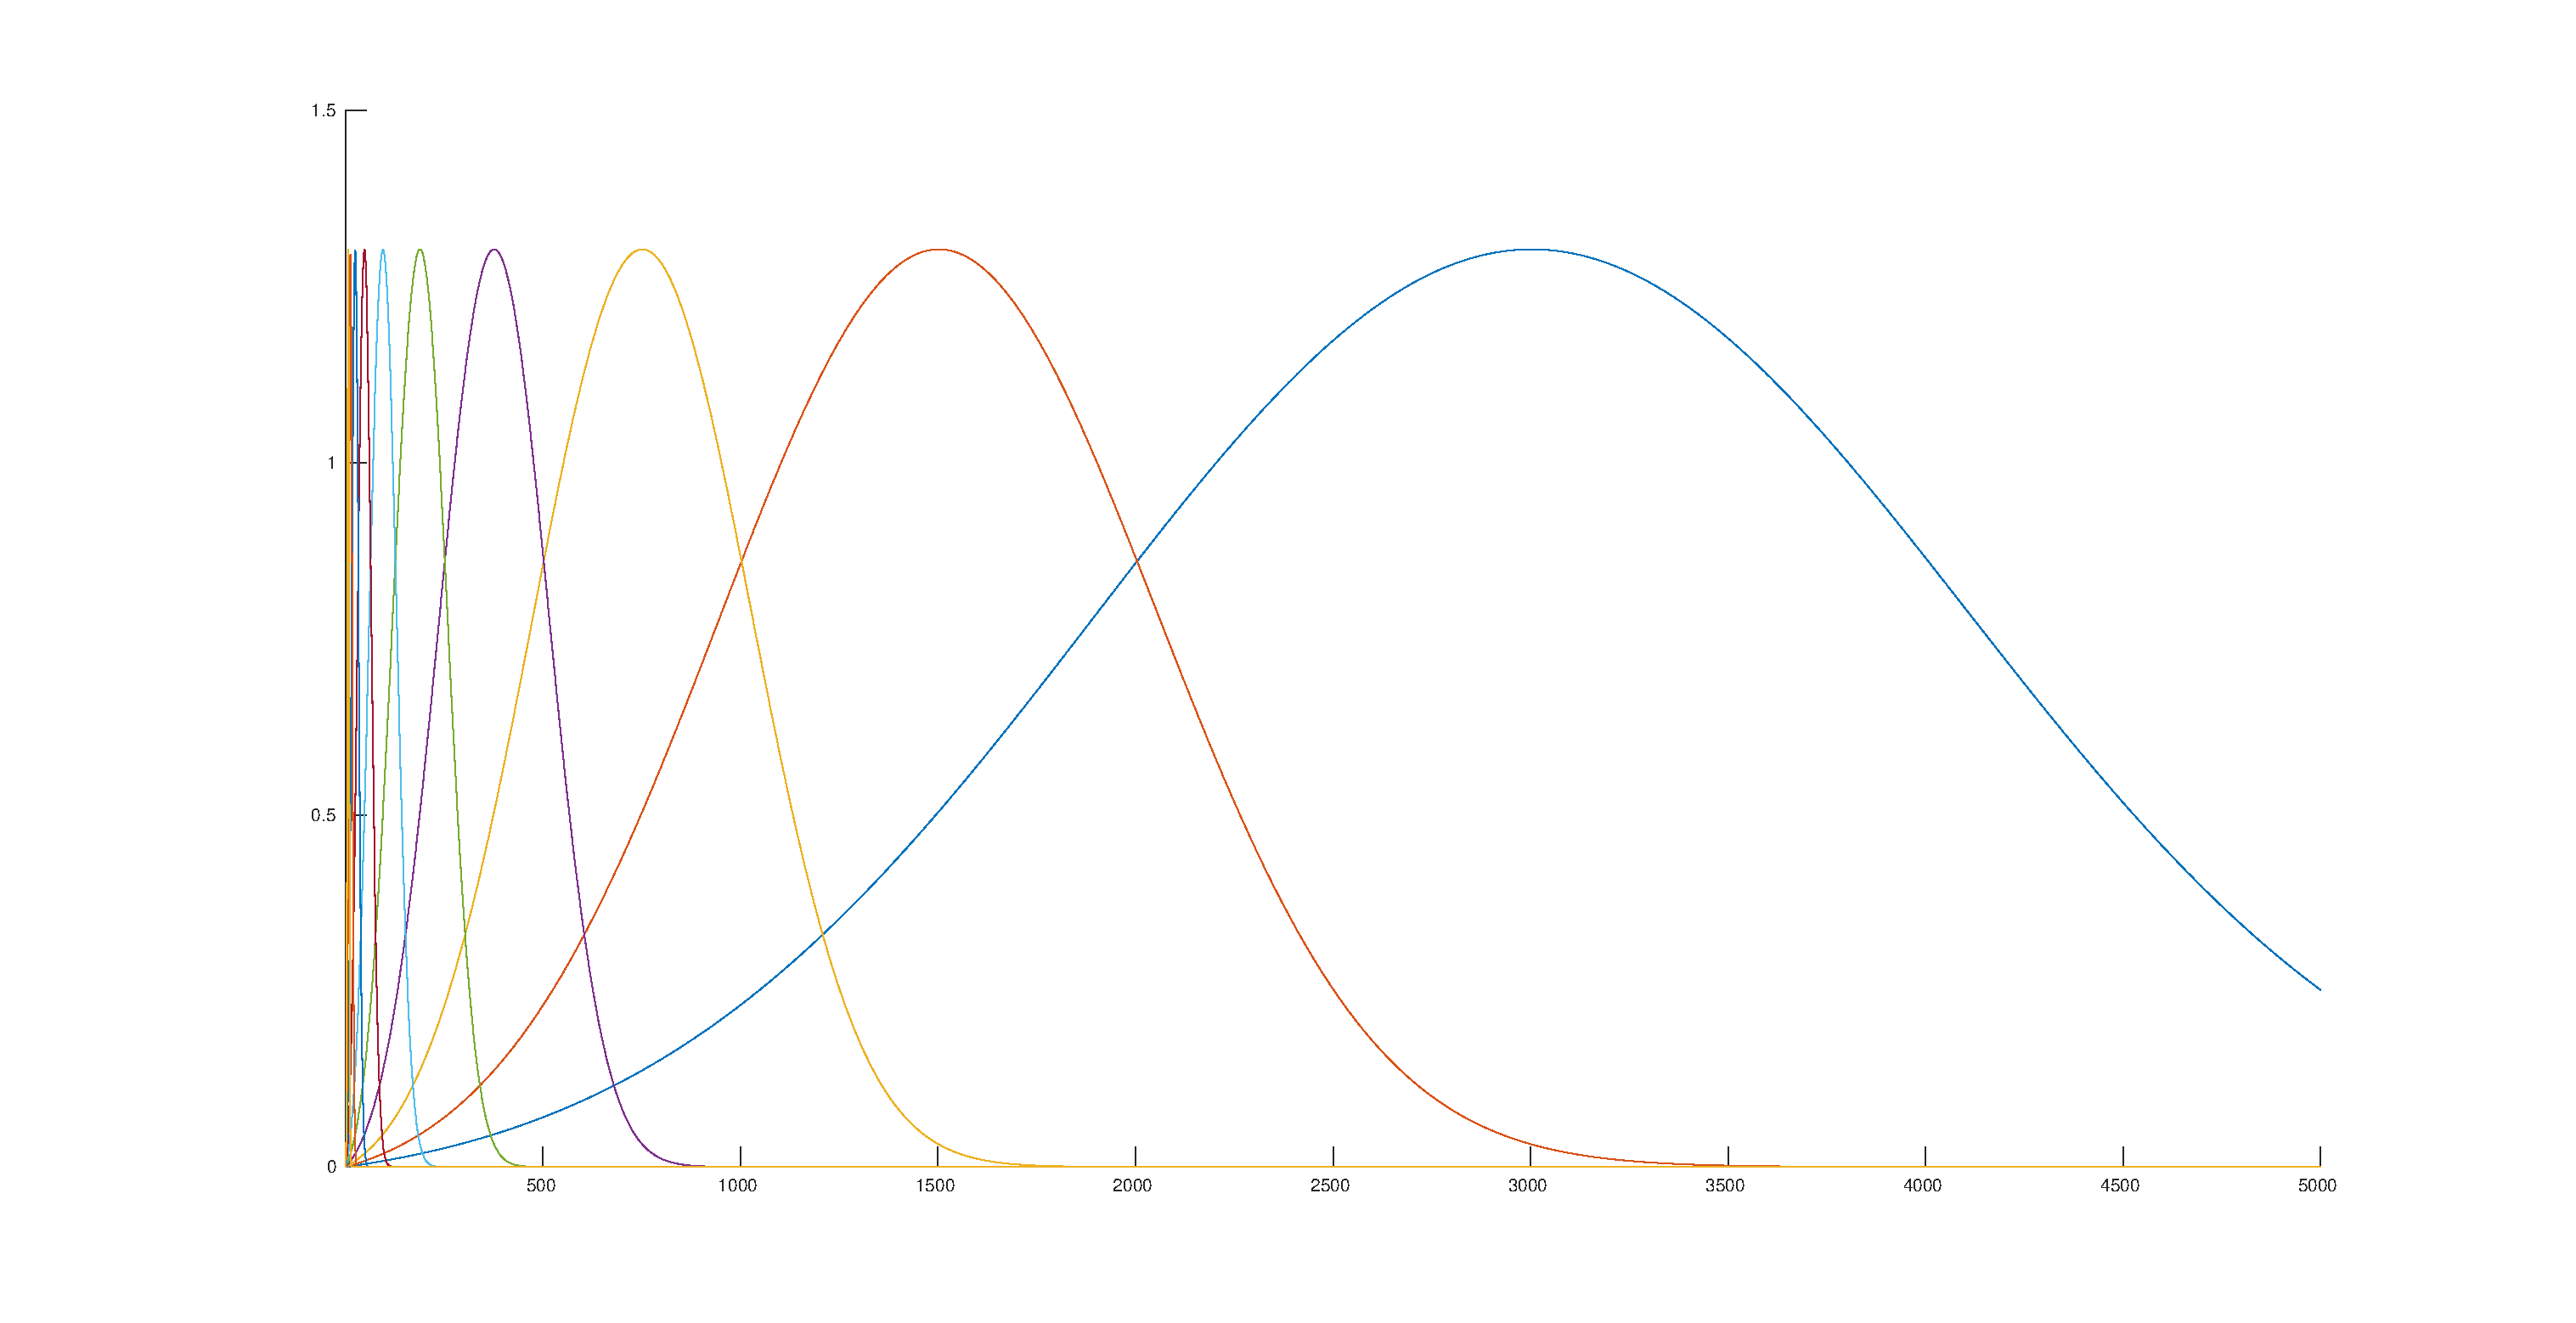
\includegraphics[width=0.9\textwidth]{img/scatter_filters_2.eps}
		\caption{Second stage.}
	\end{subfigure}
	\caption{The Morlet wavelet filterbanks.}\label{fig:filters}
\end{figure}

The mother wavelet $\psi$ may only be dilated up to the maximum scale $M-1$, resulting in 2 wavelets $\psi_{m_0}, \psi_{m_1}$. The parameter $M$ determines the maximum wavelet time support $a^M=T$,
thus the low-pass filter $\phi_M$ covers the interval $[-\pi a^{-M},\pi a^{-M}]$ and represents the length of averaging window over a neighborhood of $t$. 
In this work, we used $T=N/8=1000$ samples, which corresponds to around 60\,ms of audio. 

To improve the classification performance, scattering representation has been processed with the functions of renormalization and logarithmic transformation provided by \textit{ScatNet}. The renormalization consists in dividing second-order scattering coefficients $\mathbf{S}(x_{k,l}, m_2)$ by the first order coefficients $\mathbf{S}(x_{k,l}, m_1)$, in order to decorrelate the amplitudes at the second layer from the first layer. Log-power representation of the frequency distribution is a typical choice in many acoustical classification tasks, thus after the renormalization the logarithm of scattering coefficients is computed. 

For each audio frame, we obtain the SCAT representation $\mathbf{S}(x_{k,l}, M) \in \mathbb{R}^{D \times R}$, where $D=1+52+167=220$ is the total number of scattering coefficients (all orders combined) and $R$ is the number of time points, which is equal to 16. Finally, joining the $\mathbf{S}(x_{k,l}, M)$ for $l=1,\dots,11$ we obtain the deep scattering spectrum of the snore signal $\mathbf{S}(\mathbf{x}_{k}, M) \in \mathbb{R}^{D \times 11\cdot R}$.

\begin{figure}[h]
	\centering
	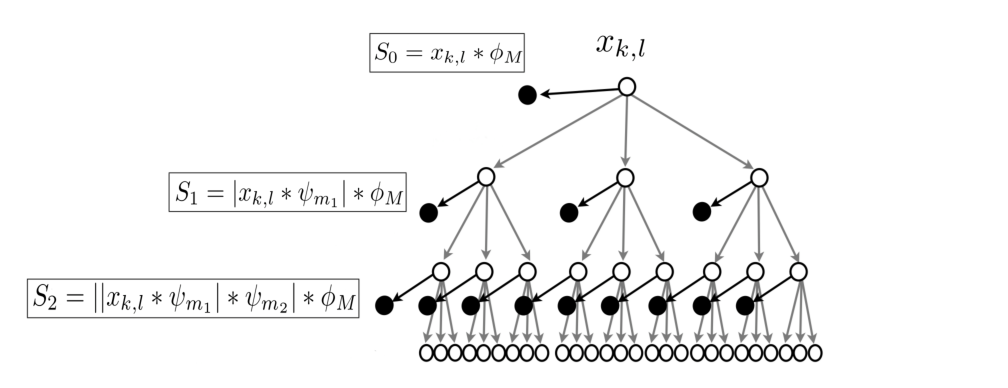
\includegraphics[scale=0.55]{img/scat_spectr_1}
	\caption[SCAT extraction tree]{The SCAT extraction tree. Picture courtesy of And\'{e}n et. al. }
\end{figure}


\subsubsection{Gaussian Mean Supervectors}
A GMS is extracted according to the following procedure. 
Let $\mathbf{s}_r = [\mathbf{S}(\mathbf{x}_{k})]_{*,r}$ the vector of the scattering coefficients of size $D \times 1$ where $r$ is the time point index, the GMM representing an UBM from the training corpus $\mathcal{T}$  is given by:
\begin{equation}\label{eq:ubm}
p(\mathbf{s}_r|\lambda) = \sum_{j=1}^{J}w_j p(\mathbf{s}_r|\boldsymbol{\mu}_j,\boldsymbol{\Sigma}_j),
\end{equation}
where $\lambda=\{w_j,\boldsymbol{\mu}_j,\boldsymbol{\Sigma}_j | j=1,2,\ldots,J\}$, $w_j$ are the mixture weights, and $p(\cdot|\boldsymbol{\mu}_j,\boldsymbol{\Sigma}_j)$ is a multivariate Gaussian distribution with mean vector $\boldsymbol{\mu}_j$ of size $D\times 1$ and diagonal covariance matrix $\boldsymbol{\Sigma}_j$ of size $D \times D$.

The mean values of the UBM model are, then, adapted with the MAP algorithm and concatenated in order to obtain the GMS:

\begin{equation}
\mathbf{\Gamma} = [\boldsymbol{\mu}_1^T,\boldsymbol{\mu}_2^T,\cdots,\boldsymbol{\mu}_J^T]^T,
\end{equation}
where $T$ denotes the transpose operator. Regardless of the length of the input snore sound, $\mathbf{\Gamma}$ is a vector of $DJ\times 1$ length. The threshold values of EM and MAP algorithms during the adaptive phase have been set both equal to 0.001, but with different number of iterations, respectively equal 1000 and 5 for EM and MAP.

\subsubsection{Multi Layer Perceptron}
In this work we exploited the Multi Layer Perceptron (MLP) architecture as DNN Classifier \cite{Rumelhart86-LRB}. The MLP is composed of an input layer with number of units equal to the dimension of the input supervector $\mathbf{\Gamma}$, followed by a stack of fully connected layers of units, namely the \textit{hidden} layers. Number of hidden layers and their dimensions have been investigated during the experimental analysis.
As non-linear activation function in the hidden layers of the MLP we employed both the hyperbolic tangent (\textit{tanh}) and the rectified linear unit (\textit{ReLU}) \cite{Nair2010}.
The output layer of the MLP is formed by four units with the \textit{softmax} non-linear function. 
The outputs of the softmax layer represent the probabilities that a sample belongs to the different classes. 

The  behavior  of  this architecture  is  parametrized  by  the connection weights, which are adapted during the supervised network training, accomplished by using the Adam algorithm \cite{kingma2014adam} for the stochastic gradient-based optimization of the crossentropy loss function. The optimizer parameters were set as follows: learning rate $lr=0.001$, $\beta_1 = 0.9$, $\beta_2 = 0.999$ and $\epsilon = 10^{-8}$. The maximum number of training epochs was set equal to 200 with an early stopping strategy in order to reduce the computational burden. 
Nevertheless, overfitting is well-know a problem affecting DNNs in particular when the number of training samples is limited. In order to prevent overfitting we investigated the use of dropout \cite{srivastava2014dropout}.

The model has been implemented in the Python language using Keras\footnote{https://keras.io/} as deep learning library with Theano\cite{2016arXiv160502688short} as back-end.



\subsection{Comparative Approaches}

Below is given a brief description of state-of-the-art approaches such as SVM classifiers and algorithms which showed the best performance at the Interspeech 2017 ComParE. They were evaluated on the blind \textit{test} set, thus they are reported for comparative aims.

\subsubsection{Support Vector Machines}

Without modifying the general structure of the algorithm for supervectors $\mathbf{\Gamma}$ computation, we compared the performance of the MLP based model with the SVMs \cite{hearst1998support}.

SVMs are binary classifiers that map an input example onto a high-dimensional feature space and iteratively searches for the hyperplane that maximises the distance between the training examples from the origin.  Given the training data $\{\mathbf{\Gamma}_{1},\dots,\mathbf{\Gamma}_{k}\}$, where $k$ is the number of observations, the class separation is performed by solving the following equation:
\begin{align}
\min_{\mathbf{w},\mathbf{\xi},\rho} & \frac{1}{2}\mathbf{w}^T\mathbf{w} + \frac{1}{\nu k}\sum_i \xi_i-\rho \\
\mbox{subject to: } & (\mathbf{w}^T \cdot \Phi(\mathbf{\Gamma}_i)) \ge \rho-\xi_i, \,  \xi_i \ge 0,
\end{align}
where $w$ is the support vector, $\xi_i$ are slack variables, $\rho$ is the offset, and $\Phi$ maps $\mathbf{\Gamma}_i$ into a dot product space $F$ such that the dot product in the image of $\Phi$ can be computed by evaluating a certain kernel function. The kernel function $K(\cdot, \cdot)$ can assume different forms \cite{bishop06}. In this work two kernel functions have been considered, the Radial Basis Function (RBF), defined as:
\begin{equation}
K(\mathbf{\Gamma},\mathbf{\Gamma}_{i}) = \exp(-\gamma \| \mathbf{\Gamma} - \mathbf{\Gamma}_{i}\|^2 )
\end{equation}
and the linear kernel, defined as:
\begin{equation}
K(\mathbf{\Gamma},\mathbf{\Gamma}_{i}) = \mathbf{\Gamma}^T\mathbf{\Gamma}_{i}.
\end{equation}
The decision values are obtained with the following function:
\begin{equation}
\label{eq:hyper}
f(\mathbf{\Gamma}) = \mathbf{w}^T \cdot \Phi(\mathbf{\Gamma})-\rho.
\end{equation}
The input vector $\mathbf{\Gamma}$ is classified as $+1$ if $f(\mathbf{\Gamma}) \geq 0$ and $-1$ if  $f(\mathbf{\Gamma}) < 0$.
In this work, the multiclass problem has been addressed using the ``one versus all'' strategy. Implementation of LIBSVM \cite{chang11} from Python library \textit{scikit-learn} has been employed both in the training and testing phases of the SVM.

\subsubsection{Weighted Kernel Classifiers}
The approach  proposed by Kaya and Karpov \cite{kaya2017introducing} exploits a decision fusion between different kernel based classifiers such as regular and weighted Kernel Extreme Learning Machine (KELM) and Kernel Partial Least Squares (KPLS) learners.
As acoustic feature representation they used Fisher Vectors (FV), which provides an encoding of local descriptors (e.g., MFCC, RASTA-PLP and their derivatives), quantifying the gradient of the parameters of the background model with respect to the data. In addition, in the final submission system they used both (FV) and the ComParE baseline feature set, which contains 6373 static features resulting from the computation of various functionals over low-level descriptor (LLD) contours.  

\subsubsection{Image-based Deep Spectrum Features}
A different approach is presented in \cite{amiriparian2017snore}, based on image classification convolutional neural network (CNN) descriptors extracted from snore spectrograms. They evaluated different well known DNN architectures typically used for image classification, such as AlexNet and VGG neural network. Both deep CNNs were previously trained on approximately 1.2 million images from the ImageNet corpus, then they compute the power spectral density on the dB power scale of the audio excerpt using Hanning windows of 16 ms width, and 8 ms overlap and they plotted the result in three different colour maps: gray, jet and viridis. The deep CNNs are fed with the spectrograms, then the neurons on the first and second fully connected layers (fc6 and fc7) are extracted as feature vectors. These feature vectors are then classified by means of an SVM model. 

\subsection{Experiments}

\subsubsection{The MPSSC dataset}
\label{ssection:MPSSCdataset}
The MPSSC dataset is composed of more than 30 hours of audio recordings captured during DISE examinations of 224 subjects from three medical centers recorded between 2006 and 2015. Recording equipment, microphone type, and location differ among the medical centers, so do the background noise characteristics. From the original signals (raw PCM, sample rate 16\,000\,Hz, quantization 16 bit) 843 early identifiable, single site of vibration snore events have been extracted and manually screened from medical experts.
Following the 4-class VOTE scheme, each sound file in the dataset is labelled as V, O, T, E, depending on the tissue from which snore sound originates, as shown in \figref{fig:vote}. They are respectively:
\begin{itemize}
	\itemsep1mm
	\item (V) - Velum (palate), including soft palate, uvula, lateral velopharyngeal walls;
	\item (O) - Oropharyngeal lateral walls, including palatine tonsils;
	\item (T) - Tongue, including tongue base and airway posterior to the tongue base;
	\item (E) - Epiglottis.
\end{itemize}


The dataset is divided into three subsets: \textit{train}, \textit{devel} and \textit{test}.
The number of events per class in the database is strongly unbalanced with a high preeminence of the ``Velum'' (V)-class  and ``Oropharyngeal'' (O)-class (85\% of samples) but in line with the likelihood of occurrence during normal sleep, while 10\% and 5\% of samples respectively belongs to E-events and T-snores. Details of class occurrences are shown in Table I.

\begin{table}[h]
	\centering
	\begin{tabular}{cccc}
		\toprule
		\multicolumn{4}{c}{\textbf{The Munich-Passau Snore Sound Corpus}} \\
		\midrule
		\#  \rule{10pt}{0pt}	& train  \rule{10pt}{0pt} & devel & test\\
		\midrule
		V \rule{10pt}{0pt}	& 168  \rule{15pt}{0pt} & 161 & 155\\
		O \rule{10pt}{0pt}	& 76  \rule{15pt}{0pt} & 75 & 65\\
		T \rule{10pt}{0pt}	& 8  \rule{15pt}{0pt} & 15 & 16\\
		E \rule{10pt}{0pt}	& 30  \rule{15pt}{0pt}& 32 & 27\\
		\bottomrule
		$\Sigma$  \rule{10pt}{0pt} & 282  \rule{13pt}{0pt} & 283 & 263\\
	\end{tabular}
	\caption[The Munich-Passau Snore Sound Corpus]{The Munich-Passau Snore Sound Corpus - The table shows the number of events per class in train, devel and test.}
	\label{tab:mpssc} 
\end{table}

As shown in the waveforms and the related spectrograms in \figref{fig:vote_spectrograms}, the main energy components in three of the classes are concentrated in the frequency area below around 2000 Hz. Energy and spectral distribution characteristics are similar, except for the Type T, which shows higher energy content above 2500 Hz compared to the other three.

\begin{figure*}[h]
	\centering
	\begin{subfigure}{.4\textwidth}
		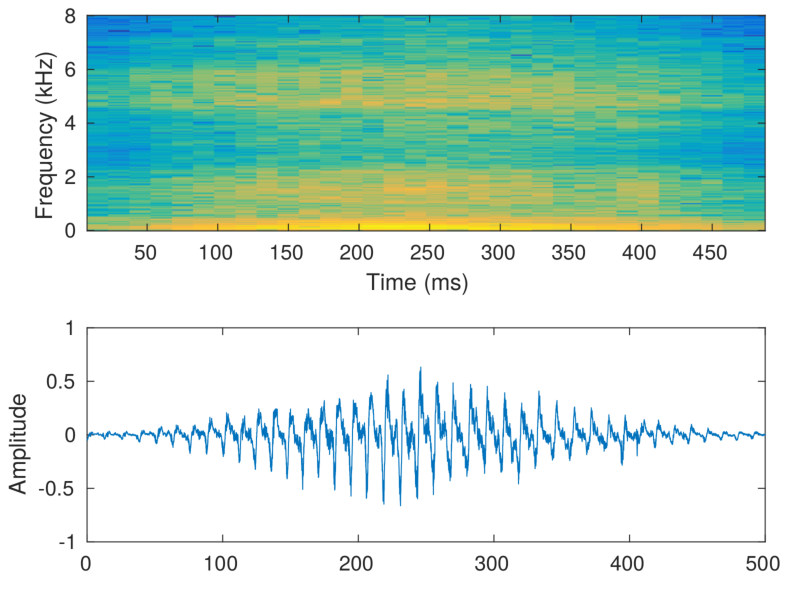
\includegraphics[width=\linewidth]{img/V_spec_crop.pdf}
		\caption{}
		\label{fig:V}
	\end{subfigure}
	\begin{subfigure}{.4\textwidth}
		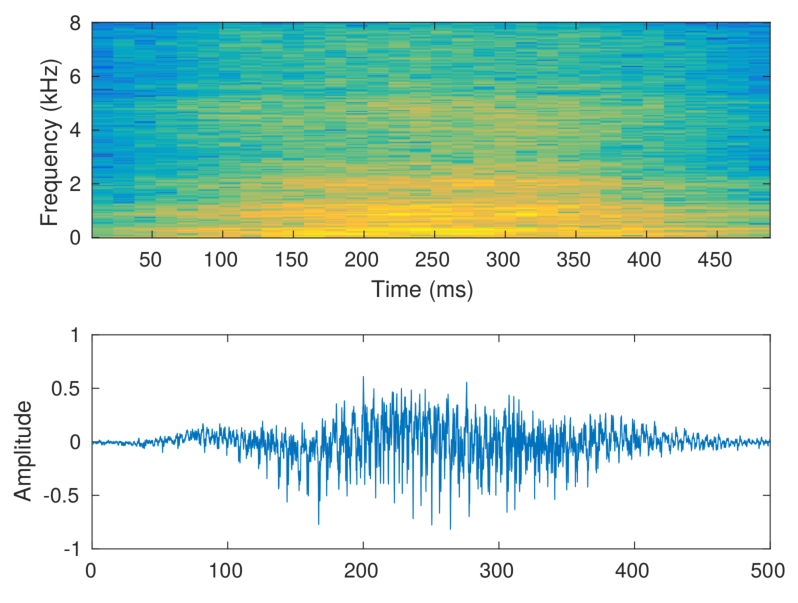
\includegraphics[width=\linewidth]{img/O_spec_crop.pdf}
		\caption{}
		\label{fig:O}
	\end{subfigure}
	\begin{subfigure}{.4\textwidth}
		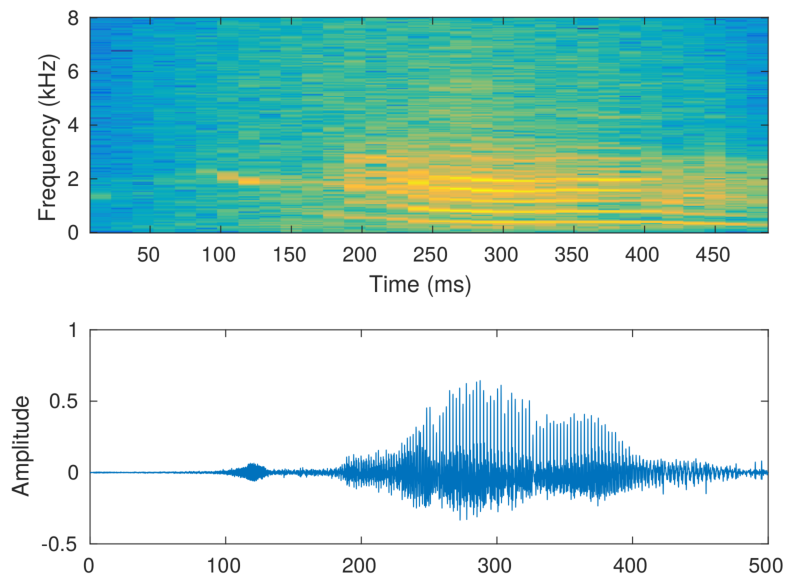
\includegraphics[width=\linewidth]{img/T_spec_crop.pdf}
		\caption{}
		\label{fig:T}
	\end{subfigure}
	\begin{subfigure}{.4\textwidth}
		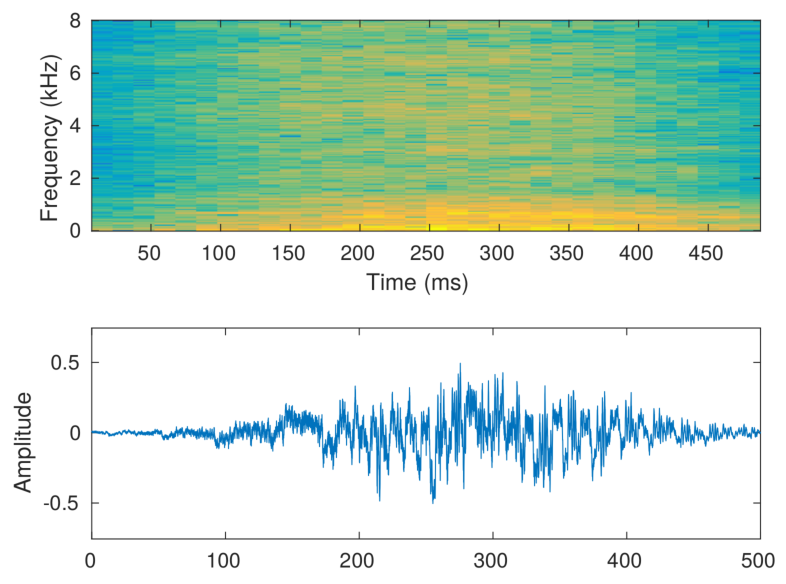
\includegraphics[width=\linewidth]{img/E_spec_crop.pdf}
		\caption{}
		\label{fig:E}
	\end{subfigure}
	\caption[Spectrograms of VOTE sounds]{Waveforms and spectrograms of VOTE events}{(a) V (velum); (b) O (oropharyngeal); (c) T (tongue base); (d) E (epiglottis).}
	\label{fig:vote_spectrograms}
\end{figure*}


\subsubsection{Experimental Setup}
According to the ComParE 2017 guidelines \cite{ComParE2017}, the performance metric for this task is the Unweighted Average Recall (UAR) which is defined as:
\begin{equation}
UAR= \frac{1}{NClass} \cdot \sum_{c=1}^{NClass}\frac{TP_c}{TP_c+FN_c}
\end{equation}

The MLP hyperparameters optimization was obtained by means of a \textit{random search} strategy  \cite{bergstra2012}.  The number of layers, the number of units per layers, the non-linear activation function and the dropout rate have been varied for a total of 400 configurations. Details of searched hyperparameters and their ranges are reported in Table II. For all of the configurations, the performance of the MLP classifier has been evaluated by varying the input supervector dimension, which depends on the number of Gaussian components used to represent the UBM $J={1,2,4,8}$. The supervector given as input to the MLP is standardized by removing the mean value of each $\boldsymbol{\mu}_j$ component and scaled by dividing for their standard deviation. 
\begin{table}[h]
	
	\centering
	\begin{tabular} {|c | c | c|}
		\hline
		Parameter & Range & Distribution\\  
		\hline
		\hline                                     
		MLP layers Nr.  & [2 - 5]& uniform \\
		\hline                                     
		MLP layers dim. & [20 - 256]& log-unifom \\
		\hline                                     
		Activation & [$tanh$ - ReLU] & uniform\\
		\hline
		Dropout Rate & [0.5 - 0] & uniform \\
		\hline
	\end{tabular}		
	\caption[VOTE Classification - Experiments]{Hyper-parameters optimized in the random-search phase for the MLP classifier, and their range.}
	\label{tab:randomsearch}
\end{table}

Regarding the SVM classifier optimization, we conducted a preliminary analysis which showed that in this task the linear kernel function provides better performance with respect to the RBF kernel.
Then, with a grid search strategy  we explored the SVM penalty parameter $C$ which yielded the best results. In particular, $C$ assumed the values $2^{-15}, 2^{-14},\ldots,2^{15}$ for a total of 30 different values. The supervectors at the input of the SVM were scaled to the range $[-1,1]$.

During the training procedure of both classifiers, different weights were given to samples belonging to different classes in order to counteract the dataset unbalancing. The weight for each class was computed on training set with the following equation:
\begin{equation}
W_c = \frac{N_{TOT}}{N_c},
\end{equation}
where $N_{TOT}$ is the total number of samples in the training set and $N_c$ the number of samples of the respective class. In this way the classes having a lower number of samples in the training set have a larger effect in the loss computing \cite{king2001logistic}. 

\subsection{Results}

The performance of the proposed algorithm has been assessed firstly by using the \textit{train} subset as training corpus and the \textit{devel} subset for evaluation. Then, the same model was trained with both \textit{train} and \textit{devel} subsets and it was evaluated on the \textit{test} subset. The results of the experiments are shown in Table III. For the sake of conciseness  only the best performances of the proposed approach are reported, comparing the results achieved with SVM and MLP classifiers on the two folds. For both \textit{devel} and \textit{test} subsets the best results are obtained with DNN based classifier.

\begin{table*}[h]
	\centering
	\resizebox{\textwidth}{!}{  
	\begin{tabular}{ c|c|c | c }
		\hline
		\textbf{Input} \rule{0pt}{10pt} & \textbf{Classifier}  & \textbf{UAR devel (\%)} & \textbf{UAR test (\%)} \\ 
		\hline
		SCAT \rule{0pt}{8pt}&  MLP [204,112,99]   & \multirow{2}{*}{53.16} & \multirow{2}{*}{72.63}\\
		+ 1 Gaussian UBM 							& with $tanh$ and dropout &							&									\\	
		\hline
		SCAT \rule{0pt}{8pt}&  MLP [249,40,21,21]   & \multirow{2}{*}{58.20} & \multirow{2}{*}{\textbf{74.19}} \\
		+ 2 Gaussians UBM 							& with $tanh$ and dropout &							&									\\	
		
		\hline
		SCAT \rule{0pt}{8pt}& MLP [235,227]   & \multirow{2}{*}{\textbf{67.14}} & \multirow{2}{*}{67.71} \\
		+ 2 Gaussians UBM 							& with $tanh$ and dropout &							&									\\	
		\hline
		SCAT \rule{0pt}{8pt}&  MLP [156,34,21]   & \multirow{2}{*}{50.30} & \multirow{2}{*}{71.32} \\
		+ 4 Gaussians UBM 							& with $relu$ and dropout &							&									\\	
		\hline
		SCAT \rule{0pt}{8pt}&  MLP [66,28]   & \multirow{2}{*}{55.89} & \multirow{2}{*}{70.18} \\
		+ 8 Gaussians UBM 							& with $tanh$ and dropout &							&									\\	
		\hline
		SCAT \rule{0pt}{8pt} & \multirow{2}{*}{SVM, $C=2^{-8}$} & \multirow{2}{*}{46.73} & \multirow{2}{*}{65.45} \\
		+ 1 Gaussian UBM & 						&							&									\\
		\hline
		SCAT \rule{0pt}{8pt} & \multirow{2}{*}{SVM, $C=2^{-10}$} & \multirow{2}{*}{46.54} & \multirow{2}{*}{65.50} \\
		+ 2 Gaussian UBM & 						&							&									\\
		\hline
		SCAT \rule{0pt}{8pt} & \multirow{2}{*}{SVM, $C=2^{-9}$} & \multirow{2}{*}{44.67} & \multirow{2}{*}{67.22} \\
		+ 4 Gaussian UBM & 						&							&									\\	
		\hline
		SCAT \rule{0pt}{8pt} & \multirow{2}{*}{SVM, $C=2^{-10}$} & \multirow{2}{*}{43.20} & \multirow{2}{*}{65.48} \\
		+ 8 Gaussian UBM & 						&							&									\\	
		\hline
		%		\hline
		%		Spectrograms + AlexNet fc7 					\rule{0pt}{8pt} & SVM	&		44.80 & 67.00 \\
		%		\hline
		%		FV and ComParE functionals	& Fusion KPLS, WKPLS, KELM and WKELM & 50.12 & 64.23  \\
	\end{tabular}
	}
	\caption[VOTE Classification - Results]{Comparative results in terms of UAR (\%) score of proposed method for MLP and SVM based classifiers for both \textit{devel} and \textit{test} subsets. Best results on each subset are shown in \textbf{bold}.}
	\label{tab:results1}
	
\end{table*}


\subsubsection{Results on \textit{devel} subset}
On this subset the best MLP topology resulting from the random search is composed of 2 hidden layers with respectively ${235,227}$ units, $tanh$ as non linear activation function and a dropout rate equal to 0.5. The network input consists of supervectors originated from UBM with 2 gaussian components, thus the input size is equal to $440 \times 1$. This architecture provides an UAR up to 67.14\%. Regarding the SVM based classifier, the best performing model on \textit{devel} subset is fed with a supervector mapped on a UBM of 1 gaussian component and with the parameter $C=2^{-8}$ obtain an UAR equal to 46.73\%.
The corresponding confusion matrices are illustrated in \figref{fig:cm_devel}, which exhibits for the MLP (\figref{fig:cm_devel_mlp}) the higher recall (80.00\%) for the minority class (T), but a moderate recall (53.12\%) for the second smallest class (E). The SVM based classifier obtains the highest recall on the (E) class, while the other classes obtain worse performance. The superiority of the DNN based classifier is motivated by its well known ability to encode in the inner structure the features of the different snore sounds highlighted by the SCAT and better distinguish the samples, notwithstanding the large unbalancing of the dataset. 

\begin{figure}[h]
	\centering	
	\begin{subfigure}{.4\textwidth}
		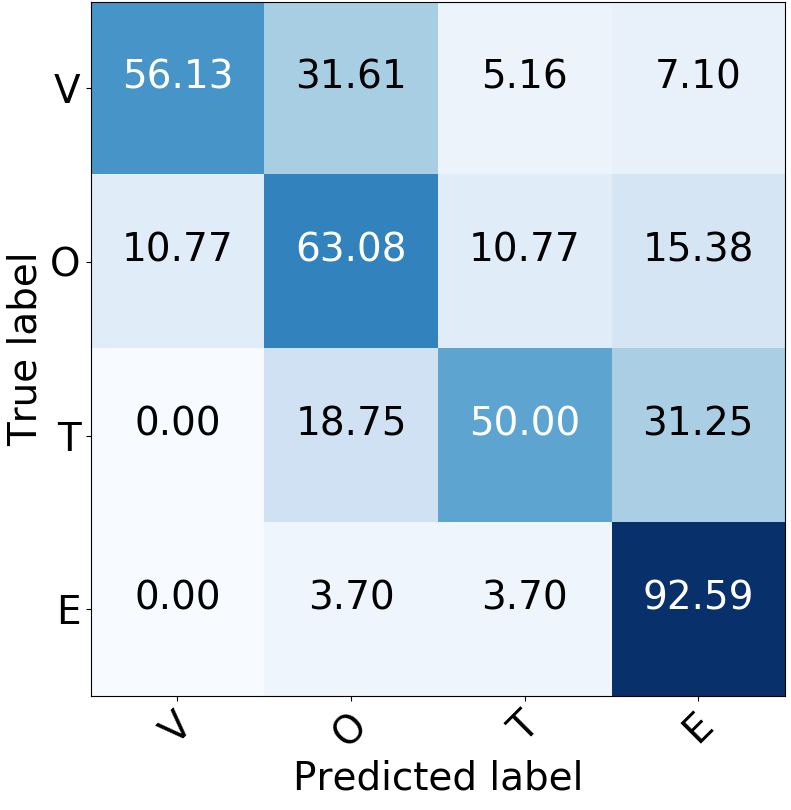
\includegraphics[width=\linewidth]{img/cm_devel_svm.png}
		\caption{}
		\label{fig:cm_devel_svm}
	\end{subfigure}
	\begin{subfigure}{.4\textwidth}
		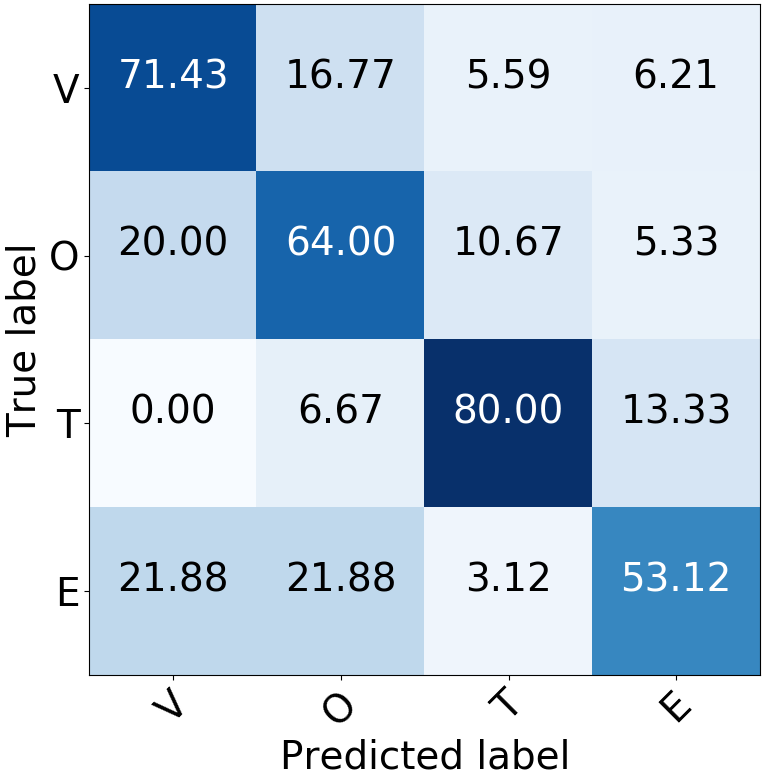
\includegraphics[width=\linewidth]{img/cm_devel_mlp.png}
		\caption{}
		\label{fig:cm_devel_mlp}
	\end{subfigure}
	\caption[VOTE Classification - Devel set results]{Normalized confusion matrix of best performing models on \textit{devel} subset. (a) SVM Classifier, (b) MLP Classifier.} 
	\label{fig:cm_devel}
\end{figure}


\subsubsection{Results on \textit{test} subset}
The network topology achieving the absolute best results optimized on \textit{test} subset is composed of 4 hidden layers with respectively ${249, 40, 21, 21}$ units, $tanh$ as non linear activation function and a dropout rate equal to 0.5. As in the case of \textit{devel} subset the input size is equal to $440 \times 1$, consisting of supervectors originated from UBM with 2 gaussian components. This architecture shows an UAR up to 74.19\%. The SVM model which obtains the best performance is fed with supervectors mapped on 4 gaussians UBM and a parameter $C=2^{-10}$. The respective UAR is equal to 67.22\%.
The obtained confusion matrices are illustrated in \figref{fig:cm_test}. In this case the augmented number of samples has a beneficial effect on the recall score of almost all the four classes for the MLP classifier, while the performance of SVM classifier are similar to the \textit{devel} subset.

\begin{figure}[h]		
	\centering
	\begin{subfigure}{.4\textwidth}
		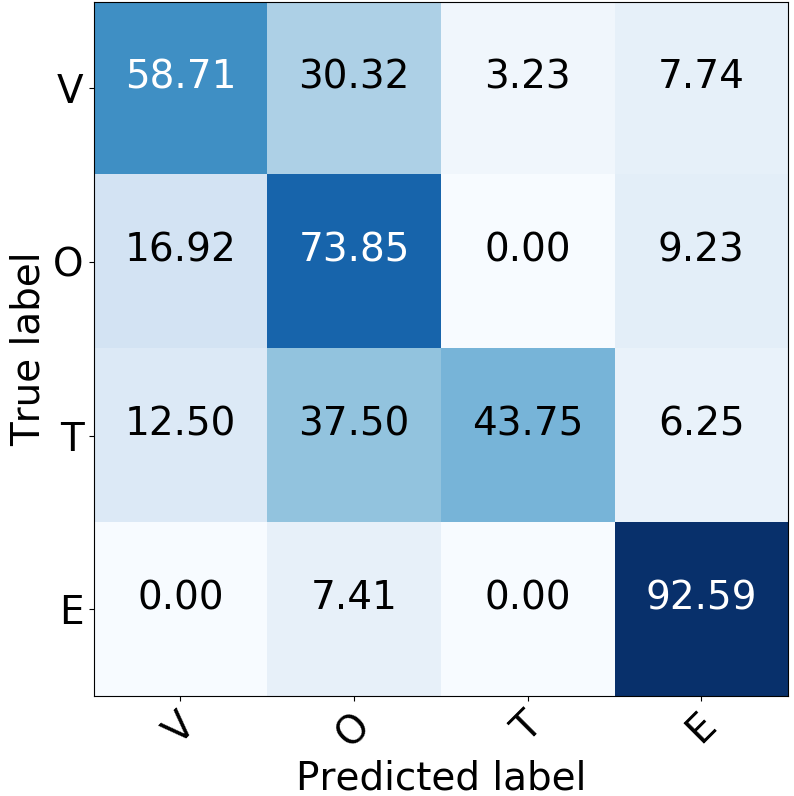
\includegraphics[width=\linewidth]{img/cm_test_svm.png}
		\caption{}
		\label{fig:cm_test_svm}
	\end{subfigure}
	\begin{subfigure}{.4\textwidth}
		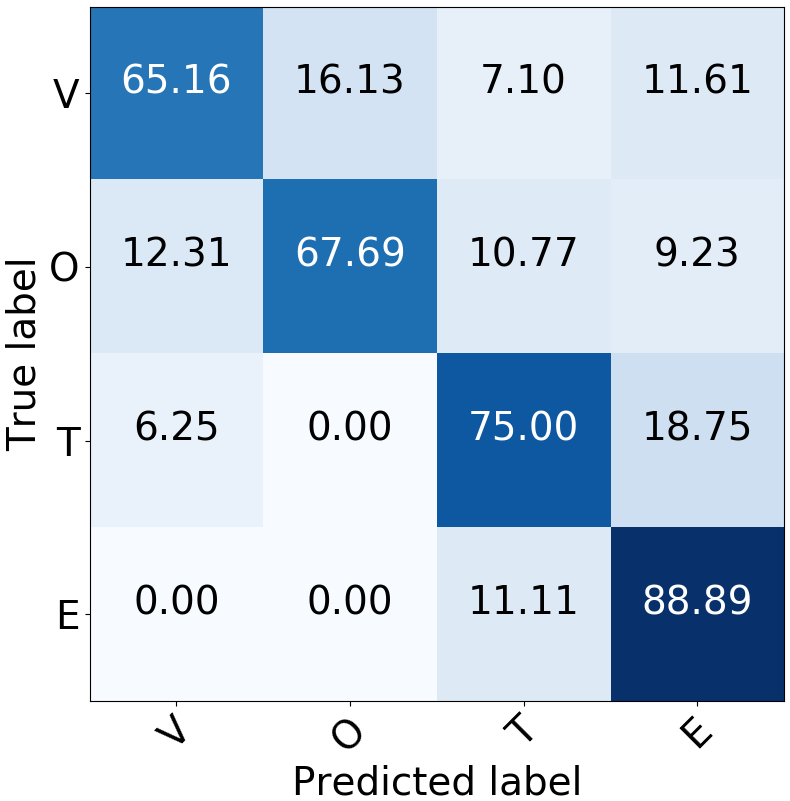
\includegraphics[width=\linewidth]{img/cm_test_mlp.png}
		\caption{}
		\label{fig:cm_test_mlp}
	\end{subfigure}
	\caption[VOTE Classification - Test set results]{Normalized confusion matrix of the best performing models on \textit{test} subset. (a) SVM Classifier, (b) MLP Classifier.} 
	\label{fig:cm_test}
\end{figure}

\subsubsection{Comparative Results}
In Table IV the best performance obtained with presented methods in \cite{kaya2017introducing}, which resulted the winner of the ComParE challenge, and in \cite{amiriparian2017snore} are reported. The best UAR score on both the subsets is provided by our proposed algorithm relying on DNN classifiers. The absolute improvement on the state-of-the-art methods on the \textit{devel} subset is remarkable, in fact we obtain in terms of UAR +17.02\%. For a fair comparison on the \textit{test} partition we have to consider the score obtained with the best model on the \textit{devel} set. In this case our proposed algorithm overcome the UAR scores of +3.48\% and +0.71\% with respect to \cite{kaya2017introducing} and \cite{amiriparian2017snore}. This results highlight that the best performance obtained on \textit{devel} set do not provide at the same time the best performance on the \textit{test} set, as it also emerged from the challenge results of reported methods. The motivation of these low generalization proprieties probably relies on the dataset splits composition and their class unbalancing. 
Anyway, the obtained performances encourage the use of SCAT as snore sound features which results to be effective. In addition, the combination of SCAT and GMS allows reduce dimension of the input vector of the classifier and to obtain an higher classification accuracy with respect to state-of-the-art methods.

\begin{table}[ht]
	\centering
	\begin{tabular}{|c|c|c|c|}
		\hline
		\multirow{2}{*}{\textbf{Input}} \rule{0pt}{10pt} & \multirow{2}{*}{\textbf{Classifier}} & \multicolumn{2}{c|}{\textbf{UAR (\%)  }}\\
		\cline{3-4}
		&  & \textbf{\textit{devel}} & \textbf{\textit{test}} \\ 
		\hline
		SCAT \rule{0pt}{8pt} &  MLP   & \textbf{67.14} & 67.71 \\
		\hline
		SCAT \rule{0pt}{8pt} &  MLP   & 58.28 & \textbf{74.19} \\
		\hline
		Spectrograms + \rule{0pt}{8pt} & \multirow{2}{*}{SVM}	& \multirow{2}{*}{44.80} & \multirow{2}{*}{67.00} \\
		AlexNet fc7						&						&						&						   \\
		\hline
		FV + 	& (W)KPLS + & \multirow{2}{*}{50.12} & \multirow{2}{*}{64.23}  \\
		ComParE functionals &  (W)KELM  & 				&						\\
		\hline
	\end{tabular}
	\caption[VOTE Classification - Comparative Results]{Comparative results in terms of UAR (\%) score of proposed algorithm with state-of-the-art methods for both \textit{devel} and \textit{test} subsets. Best results on each subset are shown in \textbf{bold}.}
	\label{tab:results2}
\end{table}


\subsection{Conclusion and Outlook}
\label{section:concl}

In this work, an approach for snore sound classification based on Deep Scattering Spectrum, Gaussian Mean Supervectors and MLP classifier has been presented. We extracted the SCAT from the audio signals and GMM-based background model was trained to map the sequence of scattering coefficients in a supervector. Classification of input snore sounds has been performed using a MLP neural network and a support vector machine with comparative aims. To assess the performance of the algorithm we conducted experiments on both the \textit{devel} and the \textit{test} subsets of MPSSC dataset.
Following the 4-class VOTE scheme, we obtained a UAR of 67.14\% on the \textit{devel} set and a respective UAR equal to 67.71\% on the \textit{test} set independently of the subject characteristics. 
The performance upper limit obtained optimizing the models on the \textit{test} set is an UAR up to 74.19\%.
The obtained results showed that the employment of the DNN based classifier in combination with SCAT is effective and a significant performance improvement with respect to other state-of-the-art approaches was registered. 
Future work will evaluate strategies of data augmentation to counteract the unbalance of the dataset. In addition, the SCAT representation of the audio signals prompts the exploitation of the 2-D Convolutional neural network (CNN) to obtain a further latent representation by means of the processing taking place in its deep architecture.
A deeper focus will be given also to the temporal evolution of the signal by means of recurrent structure, such as Long Short Term Memory (LSTM) Neural Networks \cite{graves2005framewise}. 
\newpage






%%%%%%%%%%%%%%%%%%%%%%%%%%%%%%%%%%%%%%%%%%%%%%%%%%%%%%%%%%%%%%%%%%%%%%%%%%%%%%%%%%%%%%%%%%%%%%%%%
\section{Road Surface Roughness Classification}
	
	\begin{figure}[h]
		\centering
		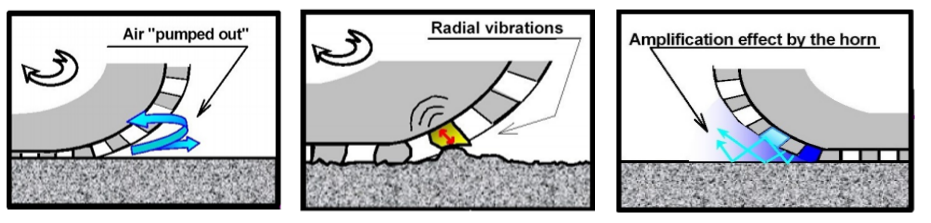
\includegraphics[width=\textwidth]{img/pompaevibrazionihorn.png}
		\caption[Tyre-Road Noises]{The tyre-road noise generation. Left:  Air pumping at the entrance of the contact patch; Center: Vibration caused by tread/block pavement impact; Right: The horn effect created by the tyre and road.}
		\label{fig:tyre-road-noise}
	\end{figure}
	
The aim of this work is to develop an automatic system for the road roughness classification. As first step was conducted an accurate state of the art analysis.	
Vehicle noise emissions depend on multiple factors, including the power unit noise, aerodynamic noise and tyre-road noise \cite{hanson2004tire}. They are all dependent on speed but have different behaviors. The power unit noise, for instance, depends on the gear engaged and the number of revolutions per minute whereas the tyre-road noise is proportional to the logarithm of the vehicle speed. The balance between these two noise contributions depends, thus, on speed. 
At low speeds the power unit noise dominates the roadside noise levels, while at high speeds the tyre/road is the predominant source of noise. In \cite{sandberg2001tyre} it is shown that  the tyre-road noise component becomes predominant with modern cars even at speeds above 30 km/h, regardless of the engaged gear. 

The tyre-road noise, results from the sum of several acoustic phenomena that concur to the noise emission. The source generation mechanism includes the following elements: 
\begin{itemize}
	\item  \textit{Tread Impact}: at the entrance of the interface between tyre and pavement (referred to as contact patch) an impact occurs as the tread hits the pavement. This impact causes vibration of the tyre carcass. 
	\item \textit{Air Pumping}: within the contact patch, the passages and grooves in the tyre are compressed and distorted. The air entrained in this passages will be compressed and pumped in and out of the passages. This  rapid exit of air can lead to sound generation.
	\item \textit{Horn Effect}: sound emitted from the tyre/road contact is reflected multiple times between the road surface and the tyre tread before it propagates further to the receiver. The tyre/road geometry has the shape of a horn. This horn shape causes a much larger radiation efficiency of the emitted tyre/road noise than in free field. This increased radiation efficiency is referred to as the horn effect. 
\end{itemize}	

\begin{figure}[h]
	\centering
	\centerline{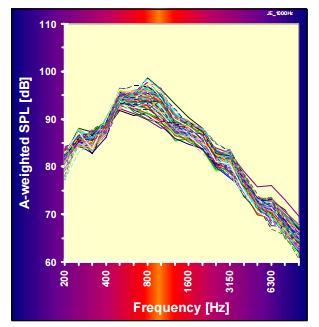
\includegraphics[width=0.45\textwidth]{img/tire.png}}
	\caption[Third-octave band noise spectra]{Third-octave band spectra obtained in TUG/VTI project for 50 different car aftermarket tyres running on the TUG drum at 90 km/h.}
	\label{fig:noise-spec}
\end{figure} 


Noise spectra have been measured on a large number of tyres (about 50) \cite{sandberg2003multi} in a cooperation project between the Technical University of Gdansk (TUG) in Poland and the Swedish National Road and Transport Research Institute (VTI). Despite a wide range of tyre types, the spectral shapes are very similar and the sound concentrates around a peak at 800-1000 Hz. 
Several studies \cite{freitas2009traffic} carried out in roads with different types of surface and age have usually shown that dense asphalt concrete and stone mastic asphalt are the ones that generate more noise contrasting with double and single porous asphalt. Porous pavements are constructed by reducing the amount of small aggregate used in the pavement
such that the pavement cannot be tightly compacted. In general, porous pavement reduces tyre/pavement interaction noise above 1000 Hz. Porosity reduces the strength of the air pumping source mechanism by preventing air compression and reduces the enhancement potential of the horn effect as shown in \figref{fig:noise-spec}. 
Some tests \cite{hanson2004tire} done in Colorado provide a preliminary understanding of the effect of pavement age on noise level. The results shows that, as expected, the older the pavement, the higher the noise level.

In this work we are interested in inferring the surface roughness by analyzing the near-field acoustic emissions of the vehicle. The surface roughness is characterized by the average size of the gravel base and the presence of filling (asphalt concrete or concrete). These elements have a large impact on the noise emission level and character. 


\subsubsection{Related Works}

A recent paper \cite{DoganRoad2017}, reports on the use of Support Vector Machines for the goal of classifying several types of road (asphalt, gravel, snow, stony road) using acoustic features. The work employs an electric car for minimal impact of the engine noise on the recording and collects 30 audio fragments from different roads at a fixed speed of 20km/h. The work employs MFCC as they were shown to maximize the Kullback-Leibler distance between all the audio fragments. Classification with the MFCC and an SVM are rather high (between 92.5\% and 97.5\%), however they decrease to 67\%-89\% when noise is artificially added to the recordings (such as rain noise or the noise of another car passing by).
SVM are employed also in \cite{alonso2014board}, where the main goal, however, is the classification of the road surface wetness and the feature extraction is done with selected 1/3 octave band filters. In that work the recordings are taken in a closed circuit with an internal combustion engine vehicle.
A different approach for road dry/wet classification is undertaken in \cite{abdic2016detecting} where a dataset is built from recordings of road trips in the US lasting tens of minutes on different types of asphalt in both dry and wet conditions. The work performs classification using a Bi-Directional Long-Short Term Memory (BLSTM) neural network \cite{hochreiter1997long} and Auditory Spectral Features (ASF). The paper reports a unweighted average recall of 93.2\% as best result, with a large improvement over \cite{alonso2014board}.

These works motivate us to investigate deep learning approaches for the road surface detection problem. In-car equalization profiles may be determined on the basis of the estimated surface roughness in order to improve the listening quality in the cockpit or to obtain suggestions on the driving experience. We propose to extract audio features for the classification of road roughness in two classes corresponding to two extremes. Owing from previous works we build a corpus of data to train an efficient neural network architecture such as a Convolutional Neural Network. The dataset deals with all the issues of a real-world scenario such as the presence of cars passing by, of a combustion engine and the varying speed. %The goal of our work is to obtain an accurate neural network model able to generalize. The neural network should have a low computational cost and should be robust to 

\subsection{Proposed Method}

\begin{figure}[h]
	\centering
	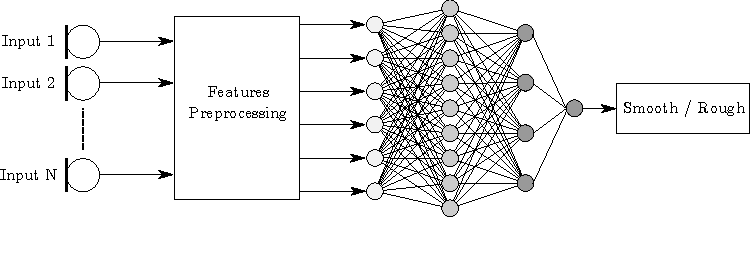
\includegraphics[width=1.0\linewidth]{img/flowchart_1.pdf}
	\caption{Algorithm Block Diagram}
	\label{fig:algoritmo-orizzontale}
\end{figure}


For the road surface classification task we propose an approach based on feature extraction, preprocessing and a classification stage based on a convolutional neural network (CNN) \cite{lecun1995convolutional}. The proposed algorithm is depicted in~\figref{fig:algoritmo-orizzontale}. The preprocessing stage works with short audio chunks to detect abrupt changes in the road surface conditions. We use Auditory Spectral Features, that are calculated in the first stage and then arranged in subsequent and non-overlapping chunks of temporal extension equal to one second in the feature extraction stage. The Neural Network stage deals with the classification and processes one block at a time.

\textbf{NDFAB: aggiungere Siamesi}

\subsubsection{Auditory Spectral Features}

Auditory Spectral Features (ASF) are acoustic features extracted from audio samples that have been introduced in \cite{eyben2010universal} and are used also in \cite{abdic2016detecting}. ASF are computed by applying the Short Time Fourier Transform (STFT) using a frame size of 30\,ms and a frame step of 10\,ms. Each STFT provides the power spectrogram which is converted to the mel frequency scale using a filter-bank with 26 triangular filters obtaining the mel spectrograms $M_{30}(n,m)$, where $n$ is the
frame index, and $m$ is the frequency bin index.

To match the human perception of loudness mel spectrograms are transformed to a logarithmic scale, according to:
\begin{equation}
M_{log}^{30}(n,m) = log(M_{30}(n,m) + 1.0).
\end{equation}
This process yields 26 coefficients, while other 26 are obtained by calculating the positive first order differences $D_{30}(n,m)$ from each logmel spectrogram, as follows:
\begin{equation}
D_{30}(n,m)  = M_{log}^{30}(n,m)-M_{log}^{30}(n-1,m),
\end{equation}
for a total of 52 coefficients for frame. The final feature vector is expanded by including the frame energy and its derivative ending up in a total number of 54 coefficients. %The block diagram of the extraction procedure is depicted in \figref{fig:ASF}. 
The features are extracted with an open-source audio analysis toolkit openSMILE v2.3.0 \cite{Eyben13-RDI} ensuring reproducibility.

%\begin{figure}[h]
%	\centering
%	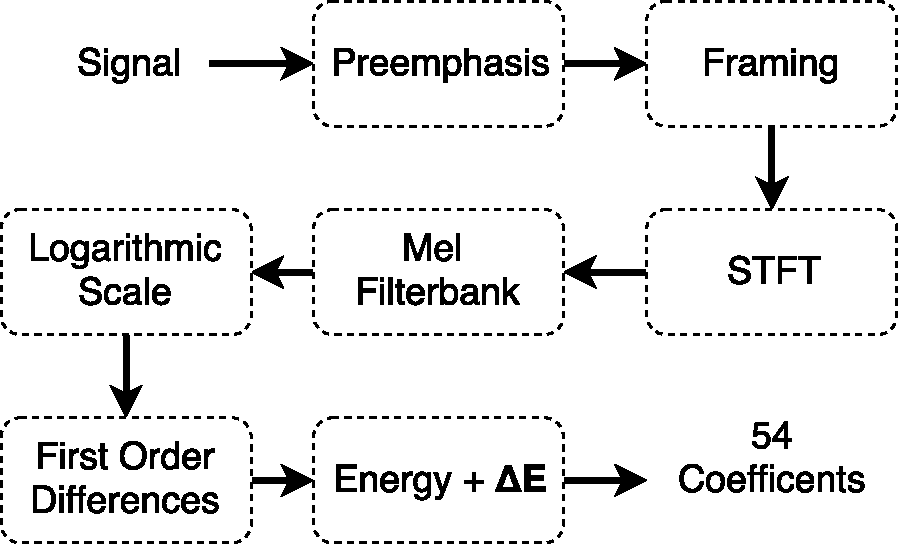
\includegraphics[width=0.5\linewidth]{img/ASF.pdf}
%	\caption{Block diagram of ASF extraction procedure}
%	\label{fig:ASF}
%\end{figure}

In order to feed the CNN, audio chunks of 1\,s are obtained from 98 feature vectors, resulting in 2D arrays of 54-by-98 values.

\subsection{Dataset}

The dataset built for this work is done with a multi-channel microphone arrangement, with the prospect of conducting different assessments at once or to exploit microphone diversity to improve the classification. More specifically, two microphones have been placed close to the rear wheels, one in front of the front left wheel, one inside the engine compartment and two inside the cockpit, close to the driver head and close to the right passenger head. The rear wheel microphones have been placed off-axis, in order to avoid dirt from the wheel and protected by the wheelhouse to reduce the effect of wind. Figure \ref{fig:car-mic} shows the positioning of all microphones. External microphones are \textit{PCB Piezotronics} model 130A24. These are IP55 microphones and they have been protected with a melamine resin foam for sound absorption to reduce the effect of wind. The internal microphones are \textit{PCB Piezotronics} model 378C20. The front-right wheel has been excluded from recordings after first informal evaluations because it picked a large amount of engine noise with respect to the other microphones. The rear-right microphone, vice versa, was found to be the best choice because the noise from the engine was the lowest and it has been used for this first evaluation. The engine compartment microphone has been used to record the engine conditions for future use. In \figref{fig:car-rr-and-fl} are shown the images of the microphones installation. 

\begin{figure}[ht]
	\centering
	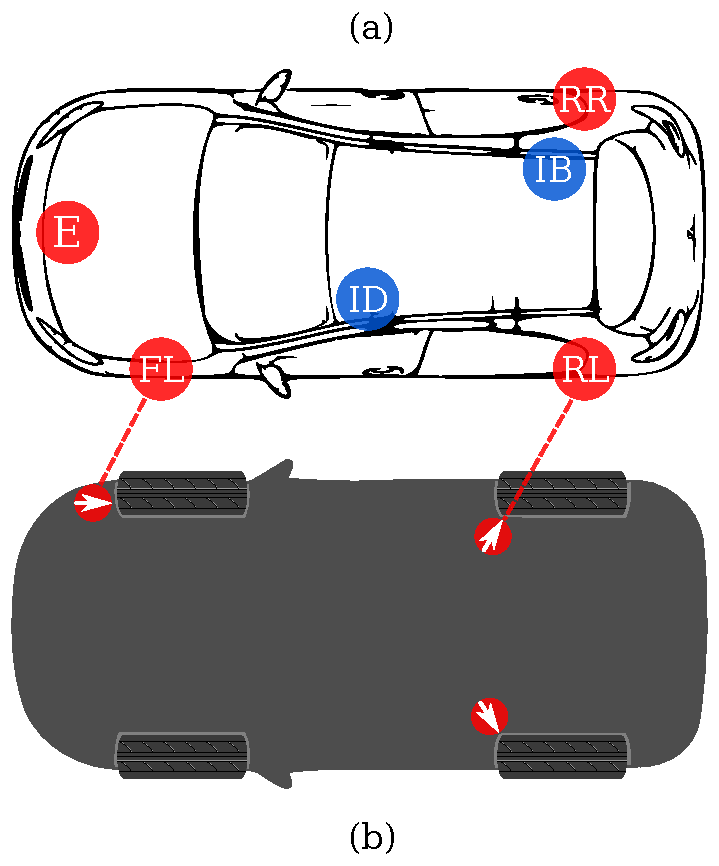
\includegraphics[width=0.6\linewidth]{img/car-mic}
	\caption[Car equipment for dataset recording.]{Positioning of the microphones in the car used to record the dataset, top view (a) and bottom view (b). The microphones are placed in the engine compartment (E), close to the front-left, rear-left and rear-right tyres (FL, RL, RR), and inside the car close to the driver or in the back seat (ID, IB). The last two microphones are \textit{PCB Piezotronics} model 378C20 type microphones, while all the others are IP55 \textit{PCB Piezotronics} model 130A24 microphones. The microphones are omnidirectional, however the arrows in (b) show how the capsule was positioned to minimize wind effect. The rear microphones are protected in the wheelhouse.}
	\label{fig:car-mic}
\end{figure}

\begin{figure}[t]
	\centering
	\begin{subfigure}[b]{0.48\textwidth}
		\includegraphics[width=\textwidth]{img/Rear-Right.jpg}
		\subcaption{Rear right tyre microphone.}
	\end{subfigure}
	\hfil
	\begin{subfigure}[b]{0.48\textwidth}
		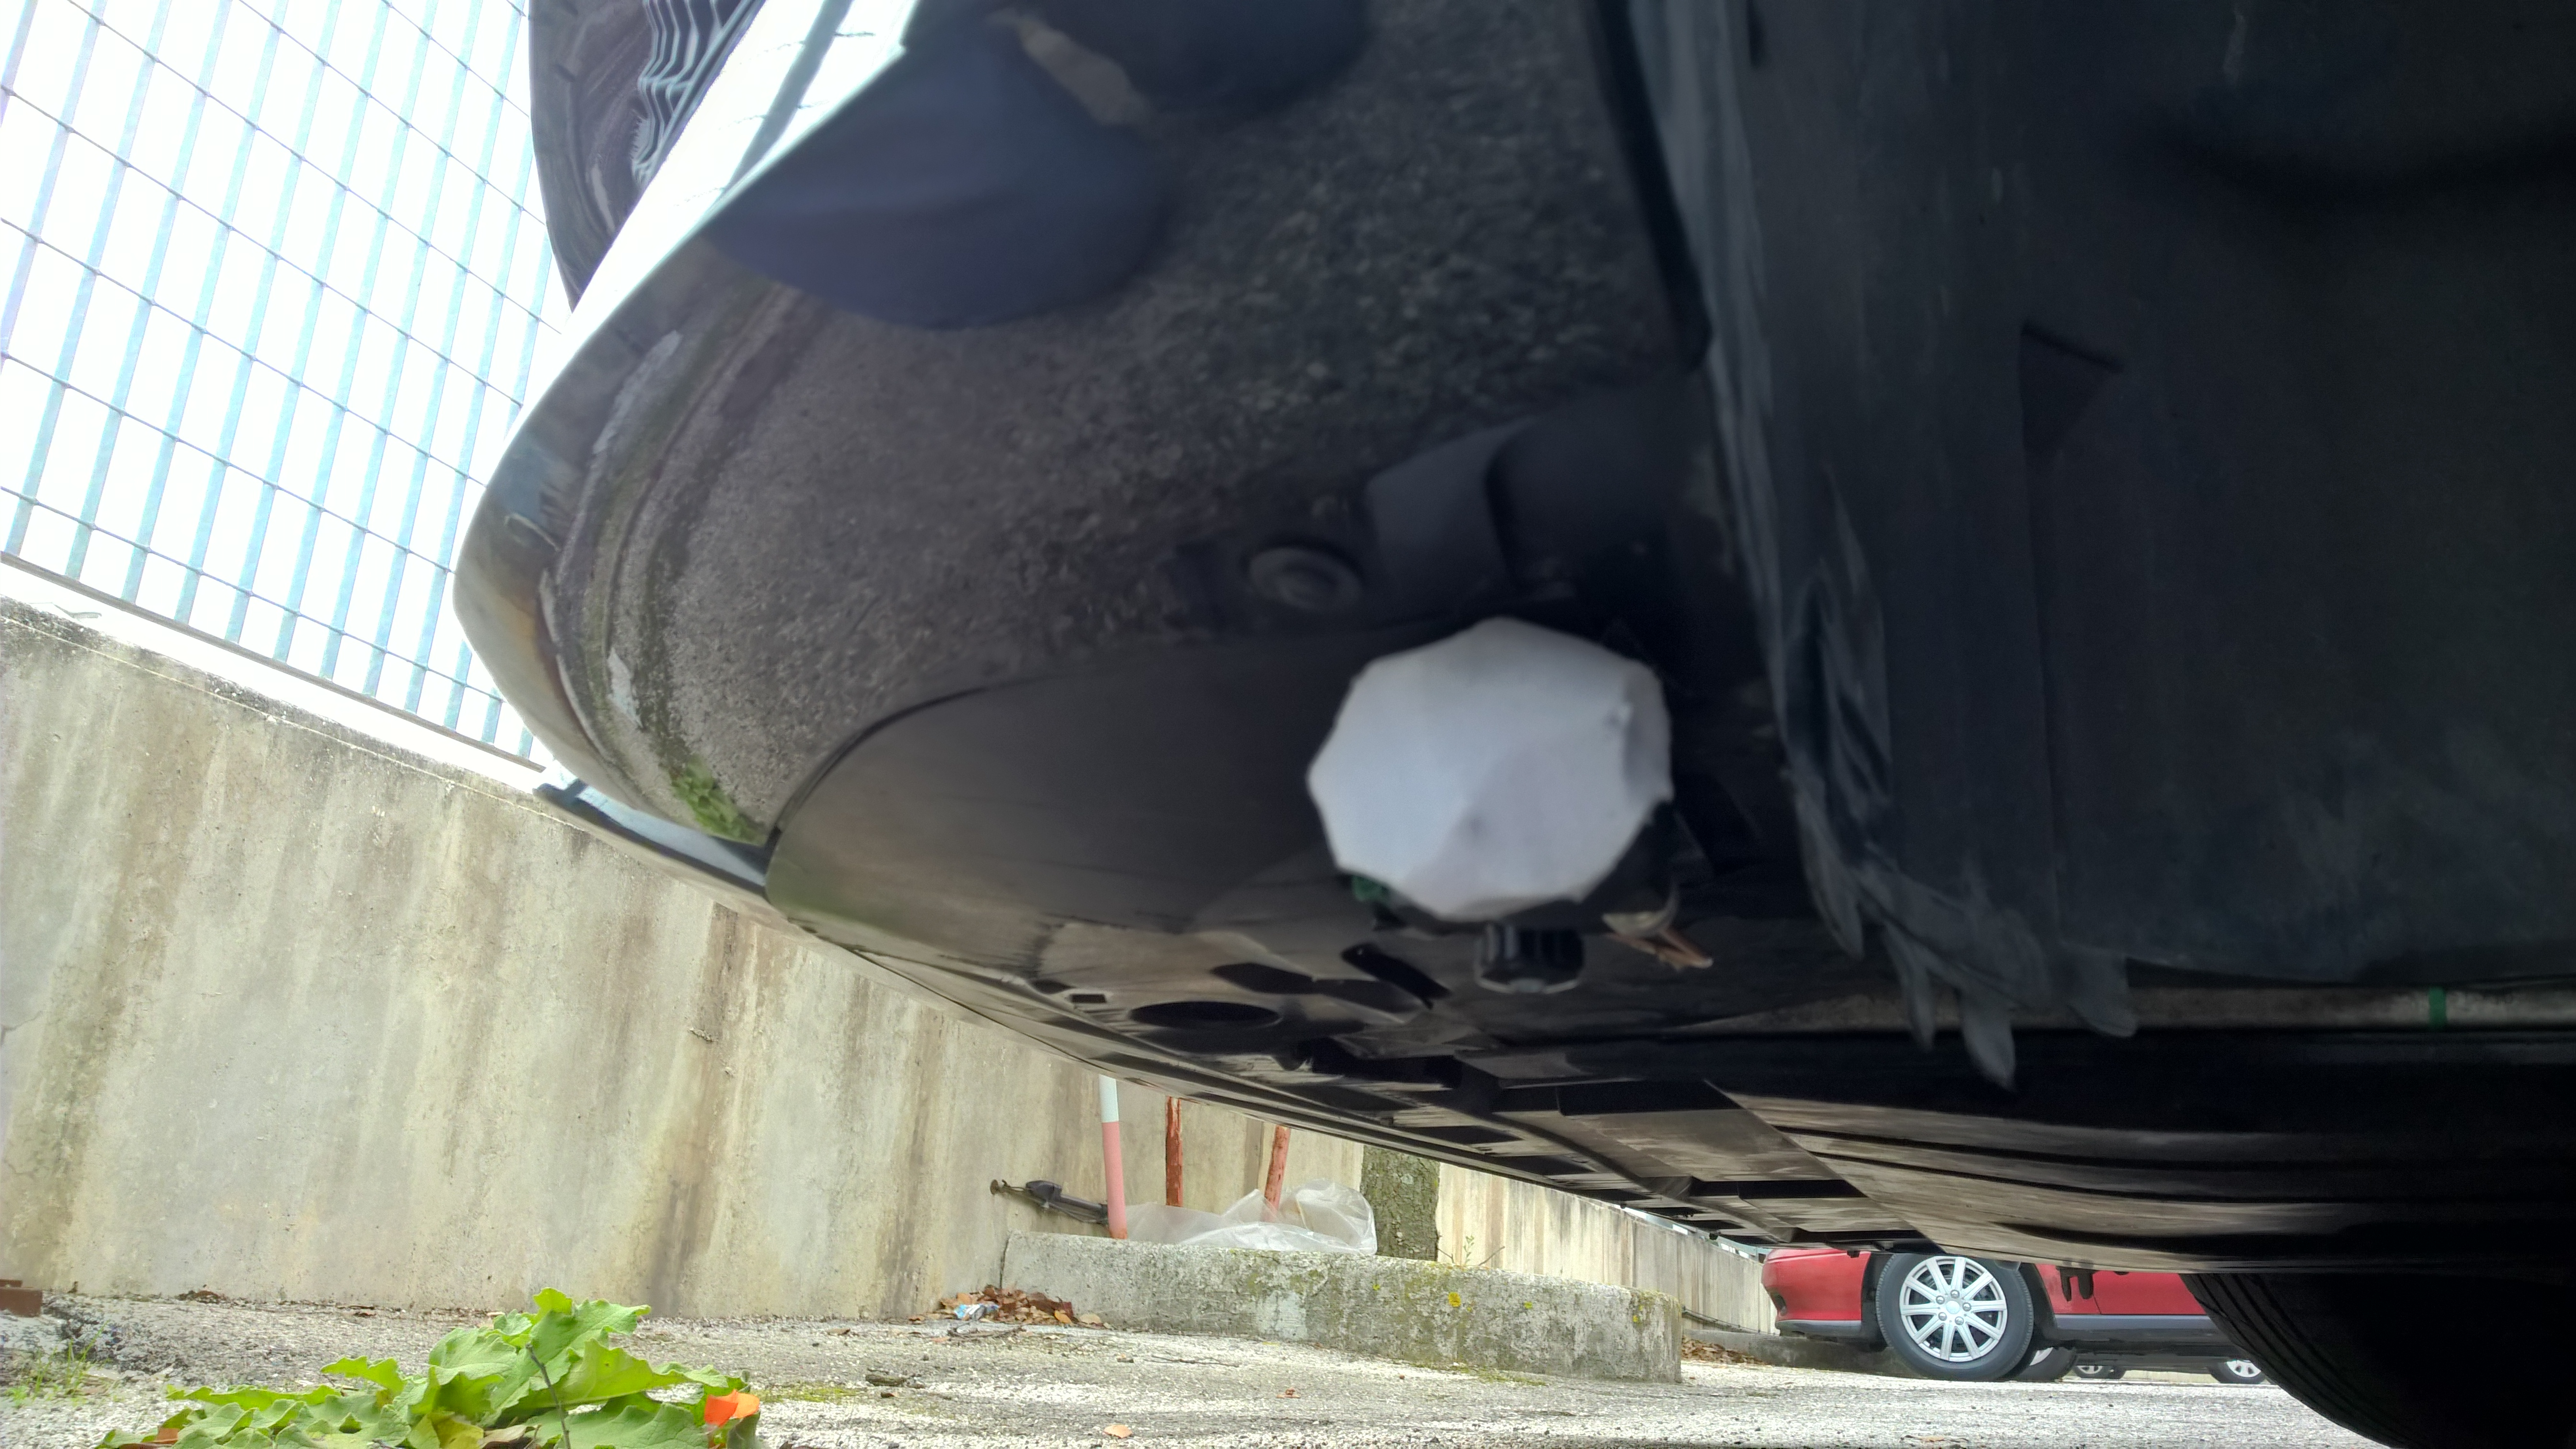
\includegraphics[width=\textwidth]{img/Front-Left.jpg}
		\subcaption{Front left tyre microphone.}
	\end{subfigure}
	
	
	\caption[Microphones positioning]{Pictures of the \textit{PCB Piezotronics} model 130A24 microphones positioned near the rear right and front left tyres, according to "RR" and "FL" red circles in \figref{fig:car-mic}. The microphones are enclosed by a melamine resin foam with open cell network structure to reduce the wind noise.}
	\label{fig:car-rr-and-fl}
\end{figure}


The car employed to build the dataset is Mercedes A Class from 2014. In addition to the audio signals, the GPS signal has been recorded to track down the car speed and position at any given time. A mobile multi-channel front end, \textit{HEAD Acoustics SQuadriga II}, has been employed as acquisition device, being able to monitor and record 8 contemporary channels at different sample rates, and to store GPS antenna and CAN bus signals as depicted in \figref{fig:car-Squadriga}.
All audio signals are sampled at 44100\,Hz, 24-bits. The external microphones used -26 dBV as input range while the interior microphones had -16 dBV as input range.
To facilitate the labelling operations, a camcorder \textit{BC Master DC10}\footnote{\url{http://www.bc-master.com/product/car-dash-camera-dc10}} was installed on the dashboard of the car. In addition to the video, it provides the speed information obtained through its own GPS antenna and it records the cockpit audio, useful for taking vocal notes while driving.

The data recorded with the \textit{HEAD Acoustics SQuadriga II} have been exported by means of the software \textit{HEAD Acoustics ArtemiS SUITE} in the uncompressed WAV audio format with a 32-bit float representation.

All recordings were taken in dry conditions in the urban and suburban areas of Ancona (Italy) with variable speed, traffic conditions and pavement roughness. Only roads that had been recently asphalted were considered and multiple takes at different speed for each road have been performed. The dataset is not perfectly balanced and is characterized by 41\% of rough road samples and 59\% of smooth road samples. For this reason a balanced version of the dataset, i.e. with equal number of smooth and rough samples, has been created by pruning excess samples for the most populated class. 
The result of the recording sessions is a 50-minutes-long dataset (41 minutes for the balanced version), with 6 audio channels and a speed channel. Labels for the roads have been annotated manually.

\begin{figure}[h]
	\centering
	\includegraphics[width=0.5\linewidth,trim={38cm 18cm 38cm 18cm},clip]{img/Squadriga}
	\caption[HEAD Acoustics SQuadriga II]{Picture of the \textit{HEAD Acoustics SQuadriga II} connected to the GPS-antenna interface.}
	\label{fig:car-Squadriga}
\end{figure}

The spectrograms from two audio samples belonging to the smooth and rough classes are shown in Figure \ref{fig:road_spectrograms}.

\begin{figure}[ht]
	\centering
	\begin{subfigure}[b]{0.48\textwidth}
		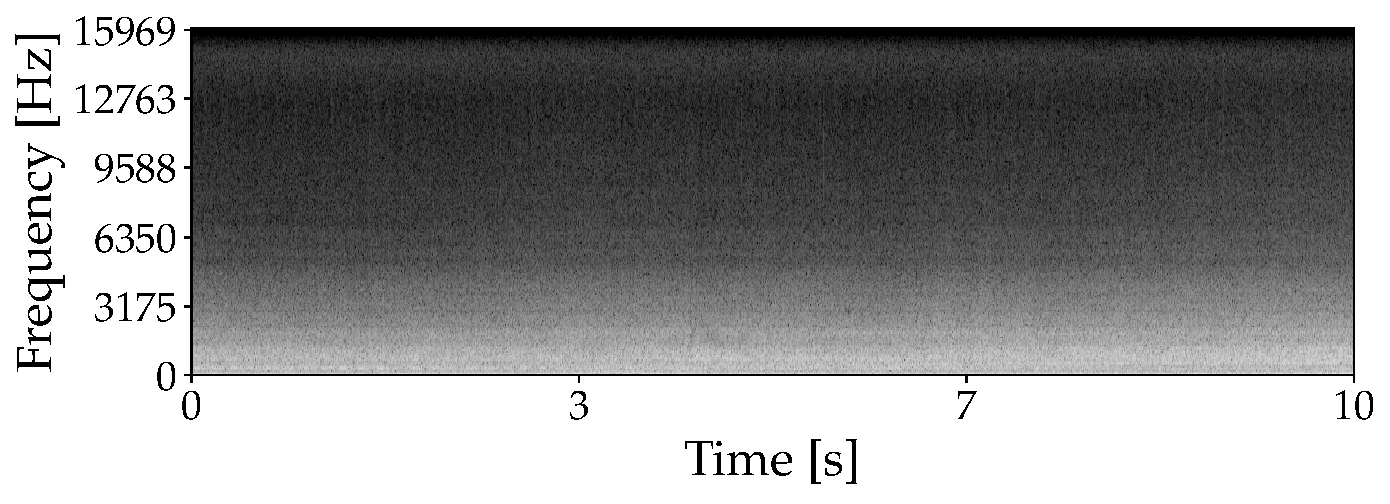
\includegraphics[width=\textwidth]{img/specgram_REC007}
		\subcaption{Smooth road.}
	\end{subfigure}
	\hfil
	\begin{subfigure}[b]{0.48\textwidth}
		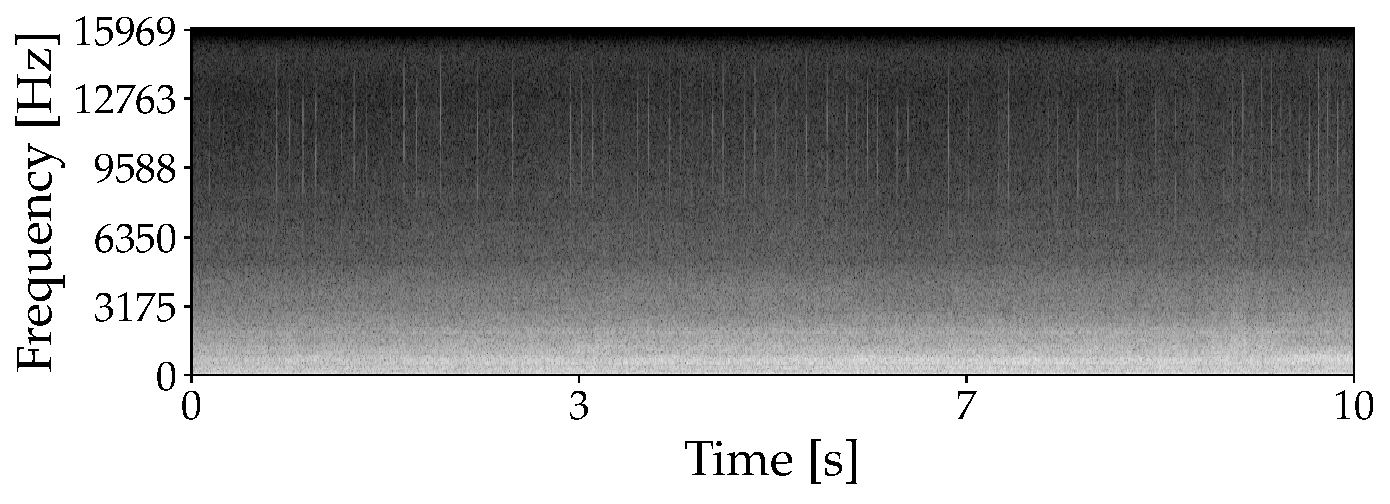
\includegraphics[width=\textwidth]{img/specgram_REC015}
		\subcaption{Rough road.}
	\end{subfigure}
	\caption[Road noise spectrograms]{Spectrograms from 10 second samples of (a) smooth urban road, (b) rough highway asphalt.}
\label{fig:road_spectrograms}
\end{figure}


\subsection{Evaluation with CNNs}  

\begin{table*}[htbp]
	\footnotesize
	\centering
	\resizebox{\textwidth}{!}{  
	\begin{tabular}{c|c|c|c|c|c}
		Configuration  & Filters        & Kernel Size                            & Strides                              & Max Pooling   & Fully Connected Layers Size      \\
		\hline
		1  & [20, 20]     & $[3\times5], [1\times2]$           & $[3\times3], [1\times2]$          & y, y    & [200, 100] \\
		2  & [15, 20]     & $[3\times5], [1\times2]$           & $[3\times3], [1\times2]$          & y, y    & [200, 100] \\
		3  & [30, 20]     & $[3\times5], [1\times2]$           & $[3\times3], [1\times2]$          & y, y    & [200, 100] \\
		4  & [15, 20, 30] & $[3\times5], [2\times2], [1\times4]$ & $[3\times5], [2\times2], [1\times4]$ & n, y, n & [300, 100] \\
		5  & [20, 20, 30] & $[1\times7], [9\times1], [3\times7]$ & $[1\times7], [1\times9], [2\times2]$ & n, n, n & [300, 100] \\
		6  & [20, 20, 30] & $[1\times7], [9\times1], [3\times7]$ & $[1\times7], [1\times9], [2\times2]$ & n, n, n & [600, 200] \\
		7  & [20, 20, 30] & $[1\times7], [9\times1], [3\times7]$ & $[1\times7], [1\times9], [2\times2]$ & n, n, n & [600, 100] \\
		8  & [54, 54, 30] & $[1\times7], [9\times1], [3\times7]$ & $[1\times7], [1\times9], [2\times2]$ & n, n, n & [200, 100] \\
		9  & [15, 20, 30] & $[3\times3], [2\times2], [1\times4]$ & $[3\times1], [2\times2], [1\times4]$ & n, y, n & [200, 100] \\
		10 & [20, 20, 30] & $[3\times3], [2\times2], [1\times4]$ & $[3\times1], [2\times2], [1\times4]$ & n, y, n & [200, 100] \\
		11 & [20, 20, 30] & $[3\times3], [2\times2], [1\times4]$ & $[3\times1], [2\times2], [1\times4]$ & n, y, n & [300, 100] \\
		12 & [30, 20, 30] & $[3\times3], [2\times2], [1\times4]$ & $[3\times1], [2\times2], [1\times4]$ & n, y, n & [200, 100]
	\end{tabular}
	}
	\caption[Road Surface Roughness Classification - Experiments]{(Best) tested configurations for CNNs. The kernel size and the stride are expressed as $[time\times\,features]$.}
	\label{tbl:config_names}
\end{table*}


Evaluations are reported after a random search of the CNN hyperparameters with different inputs and with both the balanced and unbalanced training sets. A 5-fold cross-validation procedure has been performed. The metrics have been calculated for each combination of training/testing set and then averaged to obtain the unweighted average metrics. The cross-validation has been performed disposing 64\% of the dataset to training, 16\% to validation and 20\% to test. The balanced dataset always performs worse than the unbalanced dataset, suggesting that the pruned information were important for the training stage. After initial tests, the rear-right microphone has been selected being the one with the lowest engine noise content.


In \tableref{tbl:config_names} are reported some of the best configurations tested while in \ref{tbl:cross-valid-res} are shown the best five results obtained. Best performance overall is achieved in the case of the unbalanced dataset with configuration 10, yielding an unweighted average F-measure equal to 86.00\% and an Accuracy of 87.1\%. 
This configuration is composed by three convolutional layers where the first two are square-shaped (2D), thus able to take into account both the temporal evolution and the frequency evolution of the features. The third filter is column-shaped (1D) and is able to take into account the temporal evolution only. Among the tested optimizers, Adam \cite{Kingma2015adam} provided the best results in most of the cases.

Regarding the fully-connected layers, the best results have been achieved using two layers with a number of neurons in the first layer comparable to the number of elements of the feature map obtained from the last convolutional layer. The hyperparameter search showed that oversizing the number of layers or the number of filters/neurons per layer degrades the performance.

\begin{table*}[htbp]
	\centering
	\resizebox{\textwidth}{!}{ 
		\begin{tabular}{c|cccccc}
			Configuration & Batch Size & Accuracy (\%) & F-measure (\%) & Recall (\%) & Precision (\%) & Optimizer \\ \hline
			10       & 5     & 87.10         & 86.00          & 93.08       & 79.92          & adam      \\
			5        & 5     & 86.11         & 85.19          & 93.83       & 78.00          & adam      \\
			2        & 5     & 86.18         & 85.19          & 93.38       & 78.31          & adam      \\
			1        & 1     & 85.88         & 84.87          & 93.41       & 77.76          & adam      \\
			7        & 5     & 85.28         & 83.85          & 89.04       & 79.24          & adam     
		\end{tabular}
	}
	\caption[Road Surface Roughness Classification - Results]{Top 5 configurations sorted by performance obtained in cross-validation analysis with unbalanced training classes. The configuration numbers are the same reported in Table \ref{tbl:config_names}.}
	\label{tbl:cross-valid-res}
\end{table*}


\subsection{Evaluation with Siamese Neural Networks}  

\subsection{Conclusions} 

In the present work a data-driven approach for road surface roughness classification is discussed, following seminal works proposed in the last years. The approach is based on a machine listening approach, where the tyre-road noise is analyzed and classified by means of deep neural networks. With respect to previous works a less computational-intensive neural network architecture has been chosen which also allows for on-line processing. A dataset has been created from a real-world scenario by fitting a car microphones and a GPS receiver and driving the car on different roads with varying speed, gathering a multi-channel dataset of 50 minutes. The CNN has been trained and a hyperparameter search has been done, yielding an F-measure of 86.00\% and an Accuracy of 87.1\% after a 5-fold cross-validation. These results are motivating, however there is headroom for improvement. Specifically, the average precision is lower than the average recall (79.92\% and 93.08\%, respectively), suggesting that some strategy to reduce the number of false positives is required. Unfortunately, given the very different size and complexity of the dataset, results are not comparable with previous works at the moment.

Future works may extend the proposed algorithm to process multiple microphone signals, exploiting diversity, thus reducing the number of errors due to cars passing by and other unrelated sound sources. Driving speed, extracted from a GPS receiver or from the CAN bus, may help improve the classification performance. The most challenging objective, however, would be to infer the road roughness from internal microphones, as these are nowadays available in many vehicles for echo cancellation and noise suppression and are not subject to issues such as dirt, wet, cold, etc. The main issues with this approach, however, are the cockpit isolation from the outside and the interference of speech and music with the road surface noise. Voice activity detection (VAD) \cite{Ephraim:1984,ghosh2011robust} algorithms should be employed and extended to detect the presence of music provided by the car infotainment system. Existing works based on CNN architectures \cite{wirn2016-vad,ijcnn2016-vad} could be a starting point as they could be integrated easily with the current framework and extended.


\subsection*{Acknowledgments}
The authors would like to thank ASK industries S.P.A. for financial support and technical assistance.
This work is supported by the Italian Ministry of Economic Development (MISE)'s fund for the sustainable growth (F.C.S.) under grant agreement (CUP) B48I15000130008, project VASM (“Vehicle Active Sound Management”).

We gratefully acknowledge the support of NVIDIA Corporation with the donation of the GPU used for this research.

%%%%%%%%%%%%%%%%%%%%%%%%%%%%%%%%%%%%%%%%%%%%%%%%%%%%%%%%%%%%%%%%%%%%%%%%%%%%%%%%%%%%%%

\section{Bird Audio Detection}
\section{Introduction}
\label{sec:intro}

Automatic wildlife monitoring is a key concern nowadays. Climatic changes, the effects of pollution and alteration of the ecosystems have to be closely controlled in order to be the litmus test for the future sustainable technological and political guidelines.

In this context, bird audio analysis is an important task of the bioacoustics for wildlife and biodiversity monitoring, which can easily embrace the deep learning concept.
In particular, detecting the presence of bird calls in audio recordings is a very common required first step for a framework that can perform different kind of  analysis (e.g. species classification, counting), and makes it possible to conduct work with large datasets (e.g. continuous 24h monitoring) by segmenting the data stream into regions of interests.

To encourage the research in automating this task, in 2016 Stowell et al. \cite{stowell2016bird} organized a first edition Bird Audio Detection (BAD) challenge. It has been appreciated to such an extent that a new round has been included in one of the tasks of the 2018 IEEE AASP Challenge on Detection and Classification of Acoustic Scenes and Events (DCASE). In fact, Task 3 consists  in determining a binary decision for the presence/absence of bird sounds on audio files recorded in very different conditions, comprehending dataset balancing, birds species, background sounds and recordings equipment.
Specifically, participants are asked to build algorithms that predict whether a given 10-second recording contains any type of bird vocalization, regardless of the species. 

The organizers invite to explore approaches that can either inherently generalize across different conditions (including conditions not seen in the training data), or which can self-adapt to new datasets. The deep neural network based approach we propose has the aim to counteract the generalization problem by means of an innovative learning procedure named ``capsule routing'' which has shown promising performances since it has been presented \cite{sabour2017dynamic} and also in pioneering employments in audio tasks \cite{iqbal2018capsule}.



\subsection{Related Works}
\label{ssec:related}


In very recent years, a strong growth of deep learning algorithms devoted to the acoustic monitoring has been observed. In particular, works such as \cite{mcloughlin2015low, piczak2015environmental, salamon2017deep} represent milestones, involving Convolutional Neural Networks (CNN) for audio signals detection and classification.
These deep neural architectures, combined with the increased availability of datasets and computational resources, have allowed large performance improvements, outperforming in most of the cases the human accuracy \cite{sailor2017unsupervised}. This has also motivated researchers to employ such architecture, eventually combined with recurrent units \cite{cakir2017convolutional}, in almost all of the tasks proposed in the recent editions of research challenges such as the DCASE \cite{DCASE2017challenge}. These algorithms often result among the strongest-performing systems \cite{limrare, valenti2017convolutional}.

Similar results came from the first edition Bird Audio Detection (BAD2017) challenge, which was held in 2016-2017. In this case different novel algorithms have been proposed to create robust and scalable systems able to automate the annotation process of audio sequences containing free-field recordings. The work of Grill and Schl\"{u}ter \cite{grill2017two} should be also mentioned, which obtained the highest score and which is based on CNNs trained on Mel-scaled log-magnitude spectrograms. The outcomes of the BAD2017 are reported in \cite{stowell2018automatic}.

A team at Google Brain recently has presented a new computational unit \cite{sabour2017dynamic} called ``CapsNet'' with the intent to overcome two known limitations of the CNNs: the excessive information loss caused by the pooling and other down-scaling operations and the inability to infer part-whole relationships between the elements which the deep neural network (DNN) has to detect. In fact, the layers of a standard CNN are good at detecting space-invariant features which characterize an image (or a spectrogram in the case of audio spectrograms), but are less effective at exploring the spatial relationships among features (perspective, size, orientation). Capsule routing has the aim to learn global coherence implicitly, thereby improving generalization performance. In the BAD application, it means that the DNN is driven to learn a general concept of the entities of ``bird song'' and ``background sounds'' without requiring extensive data augmentation or dedicated domain adaptation procedures, thus motivating the use of Capsules for the Task 3 of the DCASE 2018. % Challenge. 

\section{Proposed Method}
\label{sec:proposed-meth}

The proposed system is a fully data-driven approach based on the CapsNet deep neural architecture presented by Sabour et al. \cite{sabour2017dynamic}.
The novel computational structure of the Capsules, combined to the routing mechanism allows to be invariant to intra-class affine transformations and to identify part-whole relationships between data features.

The whole system is composed of a feature extraction stage and a detection stage. The feature extraction stage transforms time-varying audio signal into acoustic spectral features, then the second stage takes the feature vector as input and maps them to a binary estimate of bird song presence.
This latter stage is where we introduce the Capsule neural network architecture.
The network parameters are obtained by supervised learning using annotations of bird song activity as one hot target vector.

\subsection{Feature Extraction}

The feature extraction stage operates on mono audio signals sampled at 44.1 kHz. For our purpose, we exploit \textit{LogMels} as acoustic spectral representation, following results obtained in various audio tagging and sound
event detection tasks. Firstly, the audio signals are down-sampled to 16 kHz, because the most relevant frequency bands related to bird songs are in the range from 2 kHz to 8 kHz \cite{payne2010handbook}. Then, \textit{LogMel} coefficients are obtained by filtering the magnitude spectrum of the STFT with a filter-bank composed of 40 filters evenly spaced in the mel frequency scale. The logarithm of the energy of each band is computed to match the human perception of loudness. In the STFT computation, the used frame size is equal to 40 ms and the frame step is equal to 20 ms. 
All of the datasets contain 10-second-long WAV files, thus the resulting feature matrix $\mathbf{x} \in \mathbb{R}^{D_1\times D_2}$ has a shape $501\times40$.
The range of feature values is then normalized according to the mean and the standard deviation computed on the training sets of the neural networks.


\subsection{CapNet for Bird Audio Detection}
The architecture of the neural network is shown in Fig. \ref{fig:flowchart}. The first stages of the model are traditional CNN blocks which act as feature extractors on the input \textit{LogMel} coefficients.
After each block, max-pooling is used to halve the dimensions. The feature maps obtained by the CNN layers are then fed to the Primary Capsule Layer that represents the lowest level of multi-dimensional entities. Basically it is a convolutional layer whose output is reshaped and squashed using \eqref{eq:squashing}. The final layer, is a capsule layer and it is composed of two densely connected capsule units.
Since the previous layer is also a capsule layer, the dynamic routing algorithm is used to compute the output. The model predictions are obtained computing the the Euclidean length of each
output capsule, which represent the probabilities that an input feature vector $\mathbf{x}$ belongs to the background or the bird audio class, thus we consider only the latter as system output prediction.

\begin{figure}[htbp]
	\centering
	\includegraphics[width=\columnwidth]{imgs/flowchart}
	\label{fig:flowchart}
	\caption{Flow chart of the proposed neural network architecture.}
\end{figure}

\section{Experimental Set-Up}
\label{sec:experiment}

The network hyperparameters optimization was obtained by means of a \textit{random search} strategy  \cite{bergstra2012random}.  The number and the shape of convolutional layers, the non-linear activation function, the regularizers in addition to the capsules dimensions and the maximum number of routing iterations have been varied for a total of 100 configurations. Details of searched hyperparameters and their ranges are reported in Table \ref{tbl:hyper-params-mlp}.
The neural networks training was accomplished by the AdaDelta stochastic gradient-based optimisation algorithm \cite{zeiler2012adadelta} for a maximum of 100 epochs and batch size equal to 20 on the margin loss function. The optimizer hyperparameters were set according to \cite{zeiler2012adadelta} (i.e., initial learning rate $lr=1.0$, $\rho=0.95$, $\epsilon=10^{-6}$). It was chosen because it is well-suited for dealing with sparse data and its robustness to different choices of model hyperparameters. Furthermore no manual tuning of learning rate is required.

An early stopping strategy was employed in order to avoid overfitting. Thus if the validation score does not increase for 20 consecutive epochs, the training is stopped and the last saved model is selected as the final model. In addition, dropout and L2 (with $\lambda=0.01$) have been used as weights regularization techniques \cite{srivastava2014dropout}. 
The algorithm has been implemented in the Python language using Keras \cite{chollet2015keras} and Tensorflow \cite{tensorflow2015-whitepaper} as deep learning libraries.


\subsection{Dataset}
\label{ssec:dataset}
According to the DCASE 2018 guidelines, the performance of the proposed algorithm has been assessed firstly by using the development dataset for training and validation of the system. Then, a blind test on the provided evaluation dataset was performed with the models which achieved the highest performance and submitted to the organizers of the challenge. The complete dataset is composed of recordings belonging to five different collections. Further details are reported below: %Further details are reported in Table \ref{tab:dataset}.

\begin{itemize}
	\item ``freefield1010'': a collection of 7690 excerpts from field recordings around the world;
	\item ``warblrb10k'': a crowsourced dataset recorded with the \textit{Warblr}\footnote{https://www.warblr.co.uk/} smartphone app. It covers a wide distribution of UK locations and environments and includes weather noise, traffic noise, human speech and even human bird imitations; 8000 samples are used in the development dataset while a held-out set of 2,000 recordings from the same conditions is included in the evaluation split;
	\item ``BirdVox-DCASE-20k'': 20000 files containing remote monitoring flight calls collected from  recordings units placed near Ithaca, NY, USA during the autumn of 2015;
	\item ``Chernobyl'': dataset collected from unattended remote monitoring equipment in the Chernobyl Exclusion Zone (CEZ). A totoal of 6620 audio files cover a range of birds and includes weather, large mammal and insect noise sampled across various CEZ environments, including abandoned village, grassland and forest areas;
	\item ``PolandNFC'': 4000 recordings obtained from a project of monitoring of autumn nocturnal bird migration. They were collected every night, from September to November 2016 on the Baltic Sea coast, Poland, using Song Meter SM2 units with microphones mounted on 3–5 m poles.
\end{itemize}

%\begin{table}[t]
%	\centering
%	\begin{tabular}{|c|c|c|}
%		\hline
%		\ \textbf{Collection} \rule{0pt}{10pt} & \textbf{N. of samples}  & \textbf{Balance} \\
%		\hline
%		\hline	
%		\multicolumn{3}{|c|}{\textbf{Development Dataset}  \rule{0pt}{10pt}} \\ 
%		\hline
%		``warblrb10k'' & 8000 & 0.75 \\
%		\hline
%		``BirdVox-DCASE-20k'' & 20000 & 0.5 \\
%		\hline
%		``freefield1010'' & 7690 & 0.25 \\
%		\hline
%		
%		Total 	& 35690	& 0.5 \\
%		
%		\hline
%		\hline
%		
%		\multicolumn{3}{|c|}{\textbf{Evaluation Dataset}  \rule{0pt}{10pt}} \\ 
%		\hline
%		``warblrb10k\_test'' & 2000 & - \\
%		\hline
%		``Chernobyl'' & 6620 & - \\
%		\hline
%		``PolandNFC'' & 4000 & - \\
%		\hline
%		Total 	& 12620 & - \\
%		\hline
%	\end{tabular}
%	\caption{Details of the dataset we used for the algorithm development. The table shows the number of audio files and the ratio between positive/negative samples (if available) of each used data collection.}
%	\label{tab:dataset} 
%\end{table}

The organizers recommended a 3-way cross-validation (CV) for the algorithms development, thus in each fold we used two sets for training and the other one as validation set in order to have scores comparable with the others challenge participant.

\begin{table*}[h!]
	\centering
	\small
	\begin{tabular} {|c | c | c| c | c | c |}
		\hline
		Parameter & Range & Distribution & CapsNet1 & CapsNet 2 & CapsNet3\\  
		\hline
		\hline                                     
		CNN layers Nr.  & [1 - 4]& uniform & 3 & 4  &  4  \\
		\hline                                     
		CNN kernels Nr. & [4 - 64]& log-uniform & [64,16,8]  & [32,16,16,32] & [32,64,4,64] \\
		\hline    
		CNN kernels dim. & [3$\times$3 - 8$\times$8]& uniform & 3$\times$3 & 5$\times$5 & 6$\times$6 \\
		\hline   
		\multirow{2}{*}{Pooling dim.} & \multirow{2}{*}{[1$\times$1 - 2$\times$5]}& \multirow{2}{*}{uniform} & [1$\times$5],[1$\times$4], & [1$\times$5],[1$\times$4], &  [1$\times$4],[1$\times$2], \\
		&											  &							   & [1$\times$4]				& [1$\times$2],[1$\times$2]	&	[1$\times$2],[1$\times$2] 	\\
		\hline                                   
		CNN activation & [tanh - relu] & random choice & tanh & relu &  relu \\
		\hline
		CNN dropout  & [0 - 0.5]	& uniform & 0 & 0 & 0 \\
		\hline
		CNN L2  & [yes - no]	& random choice & no & yes & yes \\
		\hline
		\hline
		Primary Capsules channels Nr. & [2 - 8]	& uniform & 6 & 2 & 8  \\
		\hline   
		Primary Capsules kernels dim. & [3$\times$3 - 5$\times$5]& uniform & 4$\times$4 & 4$\times$4  &  3$\times$3 \\
		\hline  
		Primary Capsules dimension & [2 - 16]	& uniform & 8 & 8 & 2 \\
		\hline  
		Capsules dimension & [2 - 16]	& uniform & 2 & 15  & 10 \\
		\hline
		Capsules dropout  & [0 - 0.5]	& uniform & 0 & 0.1 & 0.3 \\
		\hline
		Max routing iterations  & [1 - 5]	& uniform & 2 & 3 & 2 \\
		\hline
		Batch Normalization  & [yes - no]	& random choice & yes &  yes  &  yes  \\
		\hline
		\hline
		Trainable Params & - & - & 113K & 282K & 424K \\
		\hline
	\end{tabular}
	\caption{Hyper-parameters optimized in the random-search phase and the resulting best performing models.}
	\label{tbl:hyper-params-mlp}
\end{table*}



\subsection{Baseline}
The baseline system is an adapted version of the method winner of the BAD2017 \cite{grill2017two}. The peculiarity of this algorithm is its double training procedure. In a first run, the network is trained on the whole training data. Binary predictions are obtained for the testing data. The more confident predictions (the ones closer to 0 or 1) are then added to the training data as so-called ``pseudo-labeled'' samples. Thus, a second training run is performed on this extended training set and the final predictions are yielded.



\subsection{Metric}
The performance metric of the DCASE 2018 on this task is the ``Area Under the ROC Curve'' (AUC). More precisely, it is a stratified AUC: the score is computed separately for each fold of the evaluation set, then the partial scores are averaged. This procedure allows to adapt the ``detection threshold'' to each dataset conditions, then the performance across datasets are combined in an explicit weighted fashion, thus the final score is not merely influenced by the number of files in each subset.


\section{Results}
\label{sec:results}
\subsection{Results on Development dataset}
Results reported in Table \ref{tab:results} show both the best performance we obtained on the single CV fold, and the best averaged AUC. We obtain a harmonic mean for AUC equal to 83.72 for a single configuration, whilst if we consider the mean of the best performing models on the single folds we achieve an AUC equal to 85.08.

%We performed the hyperparameter selection of the models with the CV procedure as described above. 
\subsection{Preview Score on Evaluation dataset}
We considered as candidates for the test on the evaluation procedure \cite{dcase2018web} both the best performing setups on the single CV folds (submission label \textbf{Vesperini\_UnivPM\_task3\_1}), and the setups with the best averaged AUC (submission label \textbf{Vesperini\_UnivPM\_task3\_2}). For the latter, we trained a new model with the same hyperparameters on the whole development dataset before performing the predictions on the evaluation dataset.


The DCASE 2018 featured a submission site where contestants could upload their predictions and compute a ``preview score'' for a subset of around 1000 files from the test set. With an ensemble of the single fold best models trained during the CV procedure we obtain an AUC score equal to 84.43, while for the model with the best averaged AUC we obtain an AUC score equal to 81.43.


\begin{table}[b]
	\centering
	\begin{tabular}{|l|c|c|c|c|c|}
		\hline
		Conf ID & Fold 1 & Fold 2	& Fold 3 & Avg & Preview Score \\
		\hline
		Baseline &	-	&	-		&	-	& 83.00 &  89.18		\\
		\hline
		CapNet1	&  \textbf{88.22} & 72.78	& 74.16	& 78.39 & -	\\
		CapNet2	&  81.77 &  \textbf{80.90} 	& 85.52	& 82.73	& 	- \\
		CapNet3	&  86.59 & 78.46	&  \textbf{86.11}	&  83.72 				& 81.83  \\
		Ensemble &	-	 & 		-	&		-			&		\textbf{85.08}  & \textbf{84.43} \\
		\hline		
	\end{tabular}
	\caption{Results on Development dataset in terms of AUC (\%).}
	\label{tab:results}
\end{table}


\section{Conclusion and Outlook}
\label{sec:conclusion}

In this paper, we have presented an algorithm for bird audio detection based on the CapsNet architecture. We feed a deep neural network which uses the dynamic routing procedure during the training with the \textit{LogMel} extracted from the audio signals in order to obtain predictions on unseen data recorded in various conditions possibly also very different from the training set. 
To assess the performance of the algorithm we conducted experiments on the development dataset from the DCASE 2018, obtaining an AUC score equal to 85.08 with respect to an AUC equal to 83.00 of the baseline system.
For future work, variants \cite{hinton2018matrix} or strategy to customize the dynamic routing can be considered.

\section{ACKNOWLEDGMENT}
\label{sec:ack}

We acknowledge the CINECA award under the ISCRA initiative, for the availability of high performance computing resources and support.
